\documentclass{article}

\usepackage{corl_2024} % Use this for the initial submission.
% \usepackage[final]{corl_2024} % Uncomment for the camera-ready ``final'' version.
% \usepackage[preprint]{corl_2024} % Uncomment for pre-prints (e.g., arxiv); This is like ``final'', but will remove the CORL footnote.
\usepackage{graphicx}
\usepackage{wrapfig2}
% ------- table part ----------
\usepackage{booktabs}
% \usepackage{graphicx}
\usepackage{caption}
% ------- theorem part ---------
\usepackage{amsthm}
\usepackage{amsmath}
\usepackage{amsfonts}
\usepackage{amssymb}

\theoremstyle{plain}
\newtheorem{theorem}{Theorem}[section]
\newtheorem{proposition}[theorem]{Proposition}
\newtheorem{lemma}[theorem]{Lemma}
\newtheorem{corollary}[theorem]{Corollary}
\theoremstyle{definition}
\newtheorem{definition}[theorem]{Definition}
\newtheorem{assumption}[theorem]{Assumption}
\theoremstyle{remark}
\newtheorem{remark}[theorem]{Remark}
%

\usepackage{algpseudocodex}
\usepackage{algorithm}

% \usepackage[disable]{todonotes}

\title{The Dark Side of VLM Rewards: Understanding and Mitigating False Positive Noise}

% The \author macro works with any number of authors. There are two
% commands used to separate the names and addresses of multiple
% authors: \And and \AND.
%
% Using \And between authors leaves it to LaTeX to determine where to
% break the lines. Using \AND forces a line break at that point. So,
% if LaTeX puts 3 of 4 authors names on the first line, and the last
% on the second line, try using \AND instead of \And before the third
% author name.

% NOTE: authors will be visible only in the camera-ready and preprint versions (i.e., when using the option 'final' or 'preprint'). 
% 	For the initial submission the authors will be anonymized.

\author{
	Sukai Huang,
    Nir Lipovetzky and 
    Trevor Cohn\thanks{Now at Google DeepMind}\\
	School of Computing and Information Systems, The University of Melbourne, Australia\\
    sukaih@student.unimelb.edu.au, \{nir.lipovetzky,
    trevor.cohn\}@unimelb.edu.au \\
  %% examples of more authors
  %% \And
  %% Coauthor \\
  %% Affiliation \\
  %% Address \\
  %% \texttt{email} \\
  %% \AND
  %% Coauthor \\
  %% Affiliation \\
  %% Address \\
  %% \texttt{email} \\
  %% \And
  %% Coauthor \\
  %% Affiliation \\
  %% Address \\
  %% \texttt{email} \\
  %% \And
  %% Coauthor \\
  %% Affiliation \\
  %% Address \\
  %% \texttt{email} \\
}


\begin{document}
\maketitle

%===============================================================================

\begin{abstract}
    Vision-Language Models (VLMs) have shown promise as reward models for reinforcement learning (RL) agents, potentially providing rich reward signals based on how well an agent's trajectory aligns with expert instructions. However, our observations reveal that RL agents trained with VLM rewards often underperform compared to those employing only intrinsic (exploration-driven) rewards, contradicting expectations set by recent work. 
	To understand this unexpected outcome, we analyze the noisy reward signals from VLMs, particularly focusing on the prevalence and consequences of false positives and false negatives. Our analysis revealed that false positive rewards of VLMs were a major factor contributing to the poor learning efficacy. 
	To address this, we developed a novel reward function, \textsc{BiMI}, that prioritizes minimizing false positive rewards while accepting a slight increase in false negatives as a necessary trade-off. Experiments demonstrate that \textsc{BiMI} substantially improves agent performance across challenging environments, highlighting the critical importance of addressing reward noise when applying VLM-based rewards to complex real-world scenarios.
\end{abstract}

% Two or three meaningful keywords should be added here
\keywords{RL, VLM-based Reward Model, Sparse Reward Environments} 

%===============================================================================

\section{Introduction}
\label{sec:introduction}

% What the problem is and why it is important to solve it
Natural language instructions are increasingly recognized as a valuable source of reward signals for reinforcement learning (RL) agents to learn complex tasks. In particular, a growing trend in agent learning involves using vision-language models (VLMs) for reward modeling. This approach measures the semantic similarity -- often quantified by cosine similarity -- between the embedding representations of an agent's behaviors (i.e., past trajectories) and the provided instructions, all within the same embedding space \citep{Kaplan2017BeatingAW, Goyal2019UsingNL, Goyal2020PixL2RGR, du2023guiding}.

% you have to give credit to the SOTA solutions, otherwise people think your problem is simple and not important

% What are the limitations of the SOTA solutions

However, we observed that RL agents trained with VLM reward models, while effective in simplified settings, often struggled with tasks involving complex dynamics and longer action horizons. This is evident in several recent works -- for instance, \citet{Goyal2019UsingNL} reported the effective use of VLM rewards in Montezuma's Revenge, a notoriously challenging Atari game. However, we observed that this success was confined to individual sub-tasks and the agent struggled when attempting to scale up to the full game. Similarly, \citet{du2023guiding} demonstrated impressive performance of VLM rewards in guiding agents within a 2D survival game. However, their study was conducted in a modified environment with a reduced observation and action space using internal game state information and manually defined macro actions. Consequently, when tested in the original, unmodified environment, their agent's performance did not exceed that of agents using only \emph{intrinsic} (exploration-driven) rewards.

The consistent underperformance of VLM-based models in complex environments, \textbf{particularly their unexpected failure to outperform even simple exploration-driven rewards}, raised significant concerns about their reliability in real-world applications. This discrepancy, where VLM reward models underperformed contrary to their perceived potential, prompted us to investigate the underlying causes of this performance gap. Our findings indicate that \textbf{noisy reward estimates} in VLMs are a key factor contributing to poor learning efficacy. We attribute this noise primarily to the approximation errors inherent in the \emph{cosine similarity metric} commonly used in these models. Specifically, our analysis focuses on two types of noise: false positives, which involve rewarding unintended behaviors, and false negatives, which occur when correct behaviors are not rewarded.

\begin{wrapfigure}{r}{0.43\textwidth}
    \begin{center}
	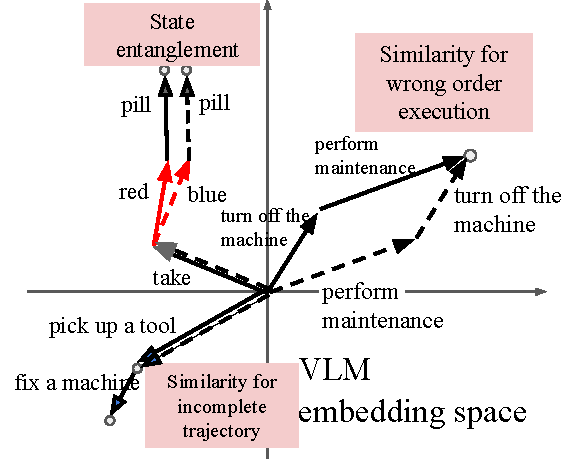
\includegraphics[width=0.43\textwidth]{figures/illustration_of_false_positives.pdf}
	\end{center}
	\caption{Schematic diagram of false positives in a VLM embedding space. The unintended agent's trajectory (dashed line) may exhibit high cosine similarity to the instruction (solid line) in the embedding space, as indicated by the proximity of their endpoints in the embedding space. Despite this apparent similarity, the unintended trajectories fundamentally fail to fulfill the intended instruction. Therefore, the rewards guides the agent towards incorrect behaviors. The figure shows three distinct cases of false positives. Refer to Section~\ref{sec:approximation_error} for more details.}
	\label{fig:false_positive_issue}
\end{wrapfigure}

We posit that false positive reward noise (see Figure~\ref{fig:false_positive_issue}) are not only more prevalent but potentially more detrimental to the learning process than false negatives, a hypothesis supported by our empirical and theoretical findings. To this end, we propose a novel reward function, \textsc{BiMI} (\textbf{Bi}nary \textbf{M}utual \textbf{I}nformation Reward). It leverages binary reward signals to directly reduce the occurrence of false positives and incorporates a mutual information term to prevent overfitting to potentially noisy signal sources. Our experiments demonstrate that \textsc{BiMI} significantly improves the learning efficacy of agents trained by VLM rewards across various challenging environments.




% Summarize contribution of the paper in precise and clear manner

\section{Related Work}
\noindent \textbf{Use of VLMs as Reward Models.}\quad VLMs have been pivotal in robotics studies, serving as reward models that guide agents to follow instructions \citep{Wang2018ReinforcedCM, Shridhar2021CLIPortWA, Mahmoudieh2022ZeroShotRS}. While most research primarily focuses on leveraging VLMs to overcome the challenge of manual reward design for complex tasks \citep{openai_faulty_rewards2016}, the impact of reward noise and its implications for policy convergence rates are often overlooked. As mentioned in Section~\ref{sec:introduction}, some work sidesteps the noisy reward problem by accessing internal state information from the game engine as well as providing predefined action macros \citep{du2023guiding, Wang2023DescribeEP}, thereby preventing the accumulation of noise over longer horizon. However, understanding the impact of reward noise from VLMs is crucial for developing reliable language interface for RL agents, as it directly affects their ability to learn effectively in real-world tasks.


% \noindent \textbf{Reward Signal from Human Preference.}\quad Recent work on Reinforcement Learning from Human Feedback (RLHF) \citep{Ouyang2022TrainingLM} also leverage human preference as a reward signal. However, our work differs in key aspects. Unlike RLHF's focus on textual outputs, our approach involves evaluating cross-modal similarities between visual and textual data in environments that require long-horizon decision-making and frequent embodied interactions, a domain not typically covered by RLHF.

\noindent \textbf{Mitigating Reward Model Failures.}\quad Research by \citet{Ghosal2022TheEO} and \citet{fufurl2024} has introduced methods to counteract unreliable reward signals from learned VLMs. These strategies involve employing a parallel exploration-based policy alongside the reward-maximizing policy, thereby reducing reliance on potentially misspecified VLM rewards. Our work contributes to this growing body of research by proposing a novel reward function that directly addresses the issue of noisy rewards in VLM-based models, complementing approaches that use exploration policies to escape local optima. Furthermore, we have tested the synergy of combining our reward function with exploration strategies, demonstrating how these approaches can be integrated for improved performance.



\section{Formal Problem Statement}
\label{sec:background}

In the context of using instructions as auxiliary guide for RL agents, we frame our task as a MDP defined by a tuple $\langle \mathcal S, \mathcal A, \mathcal T, s_0, r^{\mathit{e}}, \gamma \rangle$, where $\mathcal S$ represents a set of states $s \in \mathcal S$, $\mathcal A$ represents a set of actions $a \in \mathcal A$, and $\mathcal T(s' \mid s, a)$ describes the dynamics of the environment. $s_0 \in \mathcal S$ is the initial state, and $\gamma \in [0,1]$ is the reward discount factor. $r^{\mathit{e}}(s, a, s')$ is the environmental reward function. In this work, we focus on a sparse reward setting, where the agent receives a non-zero reward only when reaching goal states $S_G \subset \mathcal{S}$, and 0 otherwise, with $|S_G| \ll |\mathcal{S}|$. An agent's trajectory is a sequence of states and actions $\tau = \langle s_t, a_t, \ldots, s_{t+T} \rangle$, where $t$ is the initial time step and $T$ is the length of the trajectory. The objective is to learn a policy $\pi$ that maximizes the expected cumulative reward of the trajectories $\tau^\pi = \{\tau_1, ..., \tau_n \mid \tau_i \text{ induced by } \pi\}$.

A sparse reward function only \emph{realizes} a set of acceptable policies, rather than distinguishing between them more finely (as derived from \citet{Abel2021OnTE}; see Appendix~\ref{app_subsec:property_of_sparse_reward} for details). Building on this, we define the following:

\emph{(1) Policy Universe, $\Pi$:} the set of all possible policies for the MDP. 

\emph{(2) Acceptable Policies, $\Pi_G$:} the policies in $\Pi_G$ are those policies whose start-state values $V^{\pi}(s_0)$ are within a small $\epsilon$ of the optimal value, while all other policies have strictly lower values.

\emph{(3) Unacceptable Policies, $\Pi_B$:} formally, $\Pi_B = \Pi \setminus \Pi_G$, which refers to the set of policies that do not meet the near-optimal criteria and are therefore considered not acceptable.

A task instruction $L$ is a sequence of natural language sentences $L = \{l_1, l_2, \ldots, l_n\}$, where each $l_k$ induces a set of desired sub-trajectories $\tau^{l_k}$. A complete task execution is represented by a trajectory that concatenates instructions' corresponding sub-trajectories in order, traversing from the initial state $s_0$ to a goal state in $S_G$. 

\begin{wrapfigure}{0.40\textwidth}
    \centering
    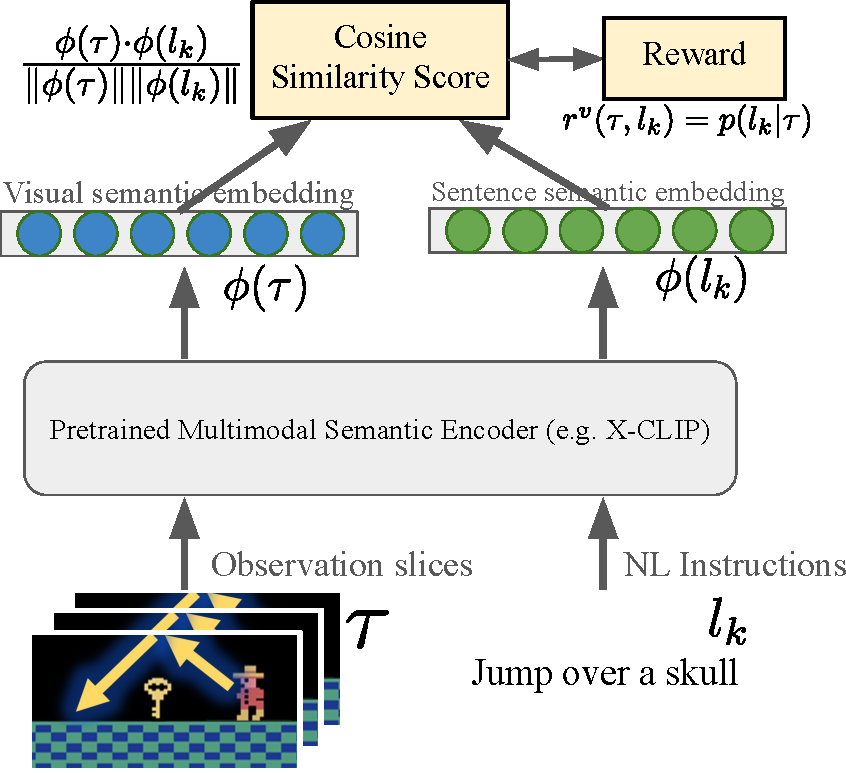
\includegraphics[width=0.40\textwidth]{figures/illustration_of_vlm_reward.pdf}
    \caption{Illustration of reward signals from a vision-language reward model}
    \label{fig:illustration_of_vlm_reward}
\end{wrapfigure}


An auxiliary VLM-based reward model provides more frequent rewards by evaluating the semantic similarity between the agent's trajectory and the specified instruction sentence. This can be formally represented as $r^v(\tau, l_k) = p(l_k|\tau)$ (see Figure~\ref{fig:illustration_of_vlm_reward}), where $r^v$ denotes the VLM-based reward function. The use of \emph{non-Markovian} reward functions in MDP environments has been well-established in the literature, particularly through the work on reward machines \citep{Icarte2018UsingRM, Corazza2022ReinforcementLW}. Such a VLM-based reward function consists of two components: an embedding encoder $\phi(\cdot)$ and a similarity function. The reward is calculated as the cosine similarity between the embeddings, which can be expressed as $\frac{\phi(\tau) \cdot \phi(l_k)}{\|\phi(\tau)\| \|\phi(l_k)\|}$.



\noindent \textbf{Reduction of Convergence Rate.}\quad To understand the effects of reward noise on policy learning, it's crucial to analyze its impact on the convergence rate. In sparse reward settings, the convergence rate -- defined as the number of training iterations needed to learn an $\epsilon$-optimal policy -- can be significantly affected by false positive rewards that are incorrectly given for policies that do not lead to the goal states.

To illustrate this, we analyze the convergence rate by measuring the probability of learning acceptable policies ($P(\pi \in \Pi_G)$) over each update iteration. The following theorem demonstrates how false positive rewards impact the convergence rate:


\begin{theorem}[Convergence rate reduction]
    \label{theo:convergence}
    In Actor-Critic algorithm, gradient ascent on $Q(s,a)\pi_{\theta_{i}}(a|s)$ pushes the next updated policy $\pi_{\theta_{i+1}}$ in the direction provided by the $Q$ value function. In the direction of maximizing $P(\pi \in \Pi_G)$, the gradient of $Q(s,a)\pi(a|s)$ can be expressed as follows:  
    \begin{flalign}
    &\nabla_\theta Q_\phi(s,a)\pi_\theta(a|s) = \textit{const} \cdot \mathbb E [G^{\pi \in \Pi_B}] \nabla_\theta \pi_\theta(a|s) \nonumber \\  &\qquad + ( \mathbb E [G^{\pi \in \Pi_G}] - \mathbb E [G^{\pi \in \Pi_B}]) P(\pi \in \Pi_G) \nabla_\theta \pi_\theta(a|s) \nonumber
    \end{flalign}
    where $\Pi_G$ is the set of acceptable policies; $\Pi_B$ is the set of unacceptable policies that follow instructions but fail to reach the goal; $\mathbb E [G^\pi]$ is expectation of the cumulative rewards by executing policy $\pi$ in one episode.
\end{theorem}

\noindent The proof is in Appendix~\ref{sec:proofofreductionofconvergence}. In this context, false positive rewards correspond to rewards assigned to policies within the set $\Pi_B$, which represents undesirable policies. Therefore, $\mathbb E [G^{\pi \in \Pi_B}]$ can be interpreted as the expected cumulative false positive rewards. This theorem highlights how the presence of $\mathbb E [G^{\pi \in \Pi_B}]$ reduce the convergence rate by: (1) introducing deviation in the policy update directions (the first term), and (2) reducing the gradient of the desired policy update (the second term). Both effects can significantly hinder the convergence process.

The issue of noisy rewards is not merely a theoretical concern; it has practical implications for the effectiveness of instruction-guided RL in real-world applications. In the next section, we will investigate how cosine similarity metric used in VLM-based reward models inevitably introduce false positive rewards. Additionally, we will empirically evaluate the impact of both false positives and false negatives on the learning efficacy of agents in sparse reward environments.

\section{Approximation Error of Cosine Similarity}
\label{sec:approximation_error}
% In non-RL domains such as information retrieval and recommendation systems, cosine similarity has been prevalent in measuring the similarity of two entities.
% However, its application in RL faces significant challenges. The sequential nature of decision-making in RL, where state transitions and action order are crucial for task completion, renders 
In this section, we will discuss two fundamental issues associated with cosine similarity scores in RL contexts: \emph{state entanglement} and \emph{composition insensitivity}. The former issue, state entanglement, refers to the metric's inability to recognize trajectories $\{\tau_1, ..., \tau_n \mid \tau_i \text{ induced by } \pi \in \Pi_B\}$ that, while being cosine similar to the target instruction in the embedding space, fail to reach the goal states in $S_G$. The latter issue refers to the metric's tendency to reward trajectories that execute the sub-tasks (corresponding to individual instruction sentences $l_k$) in an incorrect order. This is problematic in RL tasks where the specific sequence of executing sub-tasks, as defined by the order of instructions in $L = \{l_1, l_2, \ldots, l_n\}$, is crucial for reaching the goal states.

% \noindent \textbf{Scope of Discussion.}\quad While prior research, such as the study by \citet{du2023guiding}, has investigated the issue of false negatives in VLM-based reward models -- wherein the model fails to detect the correspondence between the agent's actions and the provided instructions, resulting in a lack of reward and slow policy convergence -- our study shifts the focus to the equally critical but less discussed issue of false positives. False positive rewards occur when agents receive rewards for actions that do not fulfill the intended instructions or task objectives.  We posit that these false positives are not only more prevalent but potentially more detrimental to the learning process than false negatives, a hypothesis supported by our empirical findings.
\noindent \textbf{The Issue of State Entanglement}\quad State entanglement refers to the issue where the cosine similarity metric erroneously pays more attention to lexical-level similarity while lacking comprehension of the underlying state transitions. Consequently, rewards are given to trajectory-instruction pairs that are cosine similar in embedding space but in fact result in distinct state transitions. For instance, consider the significant contrast between ``take the \emph{red} pill'' and ``take the \emph{blue} pill''. Despite their lexical similarity, they lead to vastly different states. However, the cosine similarity metric may represent them as similar due to the shared action ``take'' and shared object ``pill'', disregarding the critical difference in state outcomes. Understanding state transitions is crucial in sequential decision-making scenarios. Otherwise, rewards may be given to trajectories that lead to unintended states, resulting in the learning of unacceptable policies.

\noindent \textbf{The Issue of Composition Insensitivity}\quad Composition insensitivity in cosine similarity metrics gives rise to two issues: (1) \emph{rewarding incomplete task execution} -- cosine similarity may incorrectly reward partial task completion, as even incomplete trajectories can receive high similarity score in the embedding space. For instance, in a task to ``pick up a tool, then fix a machine,'' the model might prematurely reward the agent for merely picking up the tool, neglecting the crucial repair action. We also observed this phenomenon particularly in the Montezuma's Revenge environment, where RL agents tend to exploit the VLM reward on simpler aspects of the instruction (e.g., moving towards a direction) while avoiding the more challenging task of finally grabbing the key and escaping the room. \textbf{Eventually, it leads to suboptimal learning, as agents get stuck in local optima, repeatedly performing easier subtasks without progressing towards the ultimate goal.} (2) \emph{insensitivity to the ordering of execution} -- cosine similarity often fails to adequately penalize incorrect execution sequences. In a safety protocol requiring an agent to ``turn off the machinery, then perform maintenance,'' the metric might assign high rewards based merely on the presence of relevant actions, disregarding their order. While some large language models have become sensitive to the order of tokens \citep{su2024roformer}, the compact visual and sentence embeddings from multimodal VLMs remains largely insensitive to sequential information \citep{pham2020out}. This limitation can lead to potentially dangerous outcomes in scenarios where execution sequence is critical, such as in safety protocols or complex manufacturing processes.

Figure~\ref{fig:false_positive_issue} illustrates various scenarios where high similarity scores are erroneously assigned to false positive cases. To empirically demonstrate the issue, Section~\ref{sec:experiments_on_existence} presents experiments on false positive rewards and their impact on agent learning in sparse reward environments.

% # ! Add conceptual graph here to illustrate the false positive issues. 


\begin{figure*}[b]
    \centering
    
    \begin{minipage}{0.64\textwidth}
        \centering
        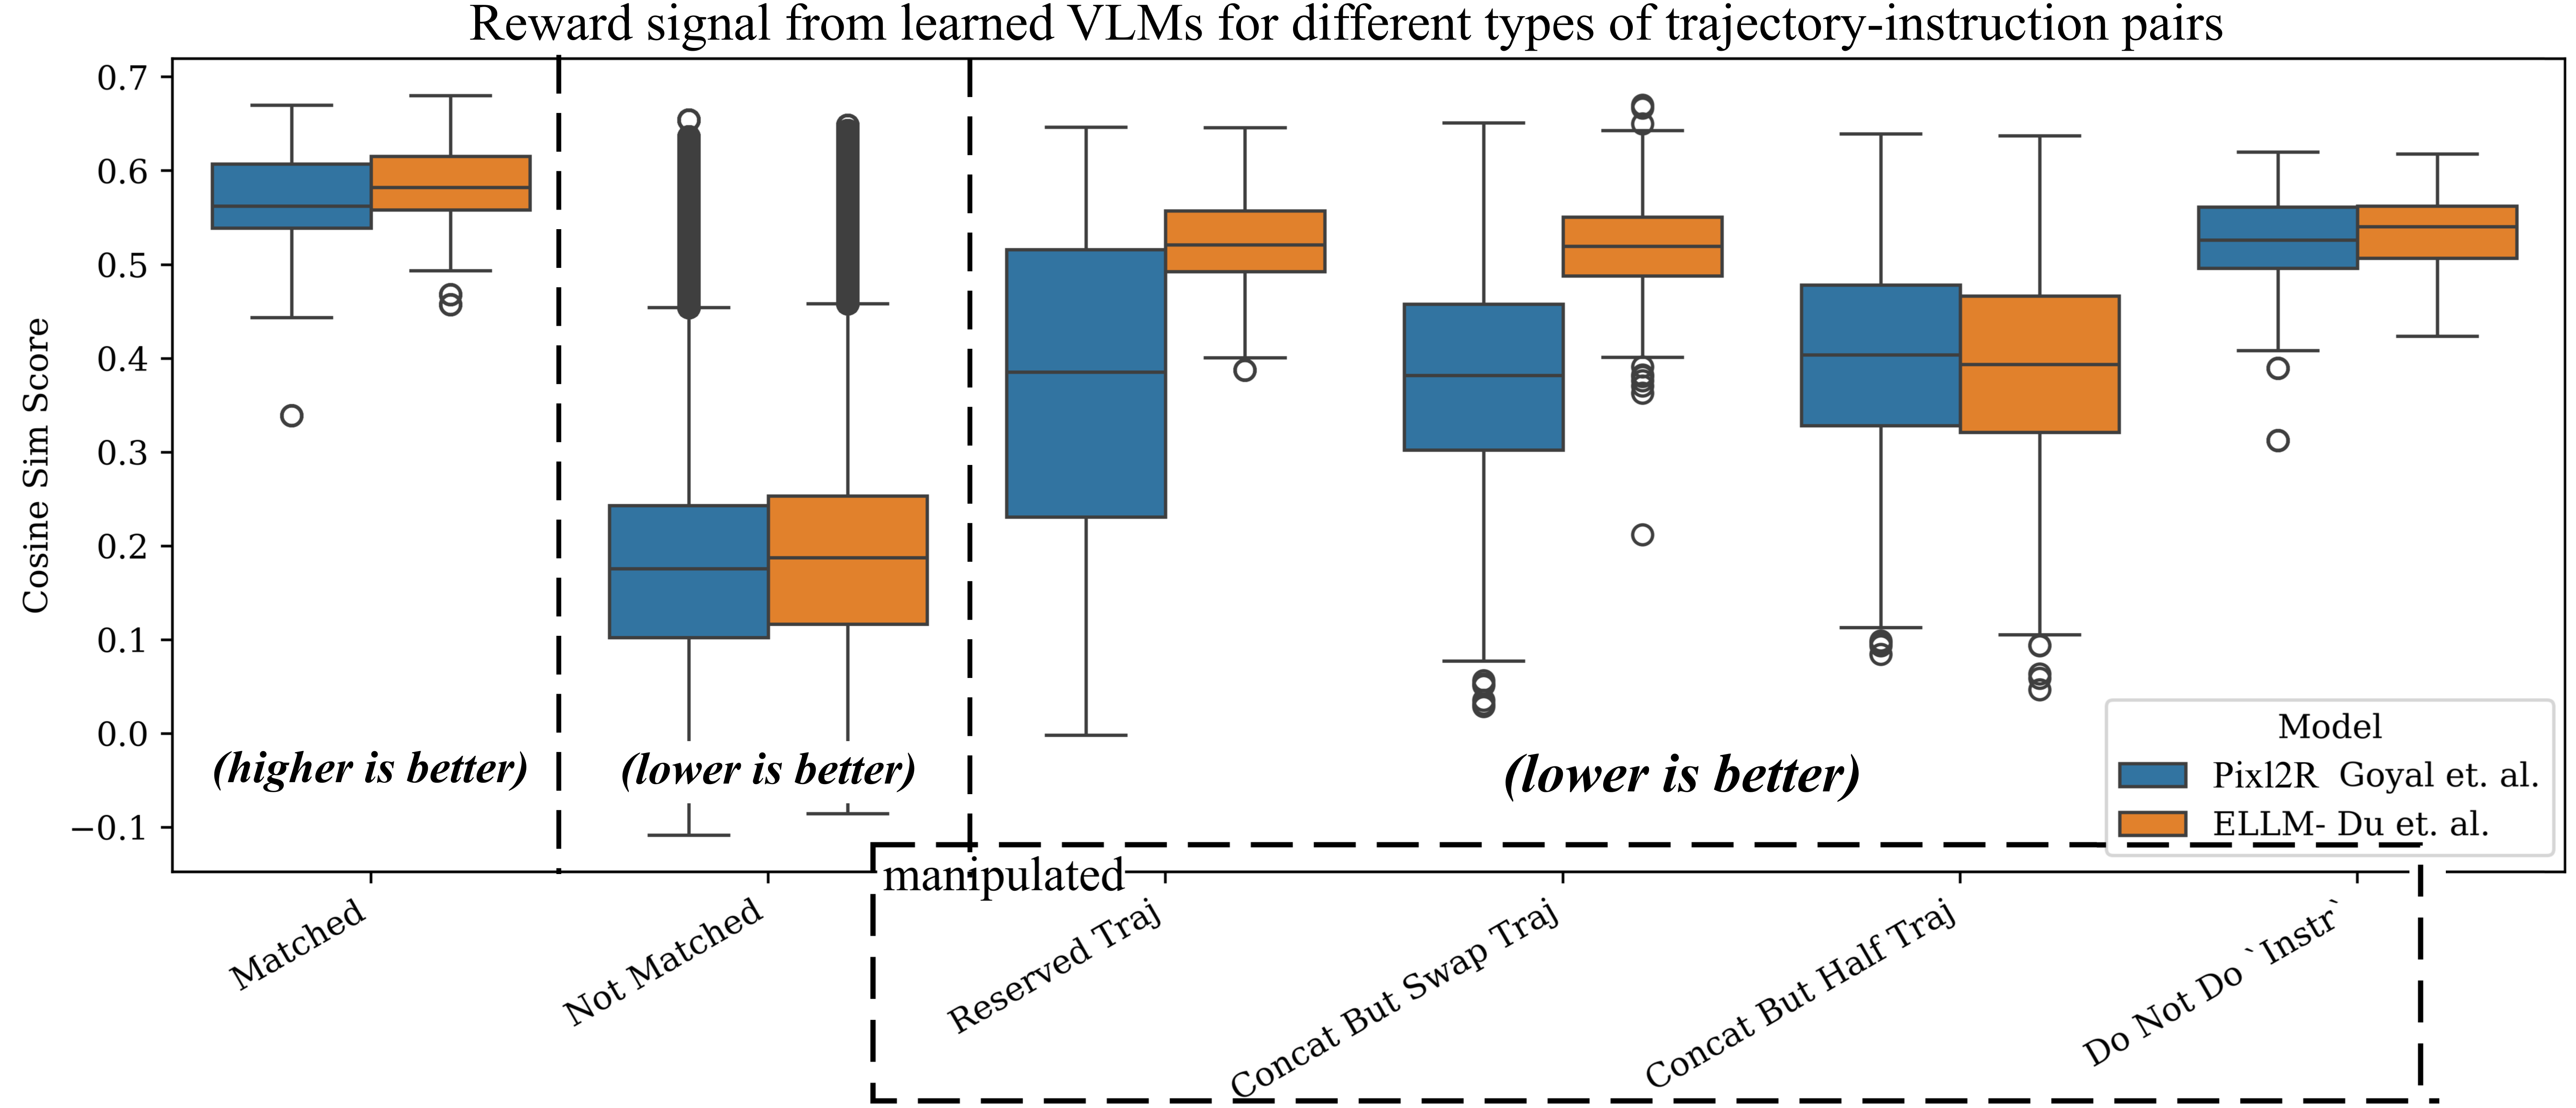
\includegraphics[width=\textwidth]{figures/cosine_sim_score_offline_eval_illu.png}
        \caption{Learned VLM models differentiate between matched and not-matched pairs, but struggle with O.O.D. cases. They incorrectly assign high scores to manipulated pairs, which should be low as the trajectories in the manipulated pairs fail the instruction}
        \label{fig:cosine_sim_score_offline_eval_illu}
    \end{minipage}
    \hspace{0.1cm}
    \begin{minipage}{0.32\textwidth}
        \centering
        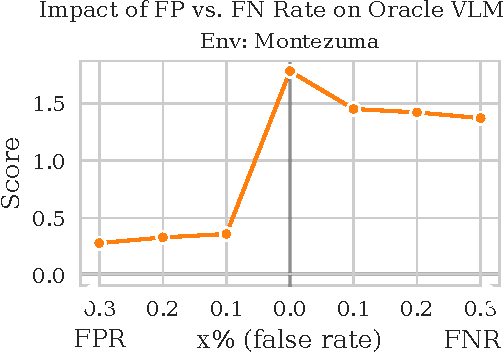
\includegraphics[width=\textwidth]{figures/montezuma_oracle_vlm_compare.pdf}
        \caption{The false positive vs. false negative oracle model. The false positive model get a more severe drop in the final training score.}
        \label{fig:FP_FN_comparison}
    \end{minipage}

\end{figure*}

\subsection{Experiments on Reward Noise Impact}
\label{sec:experiments_on_existence}
% have hypothesis stated here
Our experiments test the following hypothesis: \textbf{(H1)} The two issues of \emph{state entanglement} and \emph{composition insensitivity} exist; \textbf{(H2)} \emph{false positive} rewards are prevalent during training; \textbf{(H3)} VLM reward models lacking noise handling mechanisms underperform against intrinsic reward models in sparse reward environments; \textbf{(H4)} \emph{false negatives} may not be as harmful as \emph{false positives}.

\noindent \textbf{Setup.}\quad We evaluate these hypotheses through various challenging sparse-reward environments: (1) \emph{Crafter}, an open-ended 2D Minecraft environment \citep{Hafner2021BenchmarkingTS}; (2) \emph{Montezuma's Revenge}, a classic hard adventure game in Atari \citep{Bellemare2012TheAL}; and (3) \emph{Minigrid `Go To Seq'}, a hard task involving long-horizon navigation and object interactions \citep{chevalier2018babyai}. Two cosine similarity-based reward models were tested: (1) \emph{Pixl2R} by \citet{Goyal2020PixL2RGR}, which uses only the current video frame to determine if the goal state specified in the instruction has been reached; and (2) \emph{ELLM-}, a variant of \emph{ELLM} by \citet{du2023guiding}. Unlike ELLM, which queries instructions from LLMs in real-time, ELLM- directly uses preset expert instructions and compares them with the transition differences of the agent's trajectory. The VLM backbones used are: (1) \emph{CLIP} \citep{Radford2021LearningTV}, pretrained by image-text pairs; and (2) \emph{X-CLIP} \citep{Ma2022XCLIPEM}, pretrained by video-text pairs. To ensure high-quality finetuning data, we used internal information from the game engine to annotate expert trajectories from expert agents. To demonstrate how noisy reward signals hinder learning, we selected a strong intrinsic reward model \emph{DEIR} \citep{Zhang2021NovelDAS} for comparison. It provides auxiliary rewards based on observation novelty to encourage exploration. See Appendix~\ref{sec:implementation_details_first_stage} for detailed implementation of the experiments.

\noindent \textbf{Evaluation Metric.}\quad We used the \textbf{\emph{score}} metric adapted from the Crafter benchmark \citep{Hafner2021BenchmarkingTS} for performance evaluation, as it better captures an agent's consistent performance across multiple subtasks. This metric follows the intuitive `higher is better' principle. Unlike \emph{maximum total rewards} metric, which fail to capture consistent performance in sparse reward settings, the score metric provides a more reliable measure of learning progress.


\noindent\textbf{Reward Noise Issue.}\quad To investigate \textbf{H1}, we evaluated the models' sensitivity by examining how cosine similarity scores change for manipulated trajectory-instruction pairs. The state entanglement test involved reversing trajectories and negating instructions (i.e., ``do not do $l_k$''). The composition insensitivity test examined concatenated pairs of trajectory-instruction data. For example, given $(\tau_1, l_1)$ and $(\tau_2, l_2)$, we create a concatenated pair $(\tau_1 + \tau_2, l_1 + l_2)$. We then test two types of manipulations -- (1) swapping the order within one modality: e.g., $(\tau_2+ \tau_1, l_1 + l_2)$; and (2) truncating one modality: e.g., $(\tau_1, l_1 + l_2)$. Overall, we categorized the trajectory-instruction pairs for evaluation into three types: (1) matched pairs -- these are positive examples where the trajectory correctly corresponds to the given instruction. (2) not-matched pairs -- these are negative examples where the trajectory does not correspond to the given instruction. (3) manipulated pairs: derived from matched pairs by altering either the trajectory or the instruction. Ideally, manipulated pairs should receive low similarity scores as essentially the trajectory are not fulfilling the instruction. However, our results reveal that the reward model assigns high scores to these manipulated pairs, particularly in the ``do not do $l_k$'' case. This finding highlights the noise issue in cosine similarity-based reward models (see Figure~\ref{fig:cosine_sim_score_offline_eval_illu}). It's worth noting that the poor performance in the negation case aligns with broader challenges in natural language processing. Recent studies \citep{hossain2022analysis, truong2023language} have highlighted that negation is central to language understanding but is not properly captured by modern language models. This limitation extends to VLMs and significantly impacts their ability to provide accurate rewards in complex scenarios and instructions.

\begin{figure*}[t]
    \centering
    \begin{minipage}{0.68\textwidth}
        \centering
        
\includegraphics[width=\textwidth]{figures/h2_show_prevalence_of_noisy_rewards.png}
        \caption{The heatmap shows the cumulative rewards received at various locations, with larger circle sizes indicating higher rewards. The later figures shows the offsets between the state where rewards are given and the actual goal-reaching state. Agents are getting both issues of false positives and false negatives during training}
        \label{fig:show_prevalence_of_noisy_rewards}
    \end{minipage}
    \hspace{0.1cm}
    \begin{minipage}{0.29\textwidth}
        \centering
        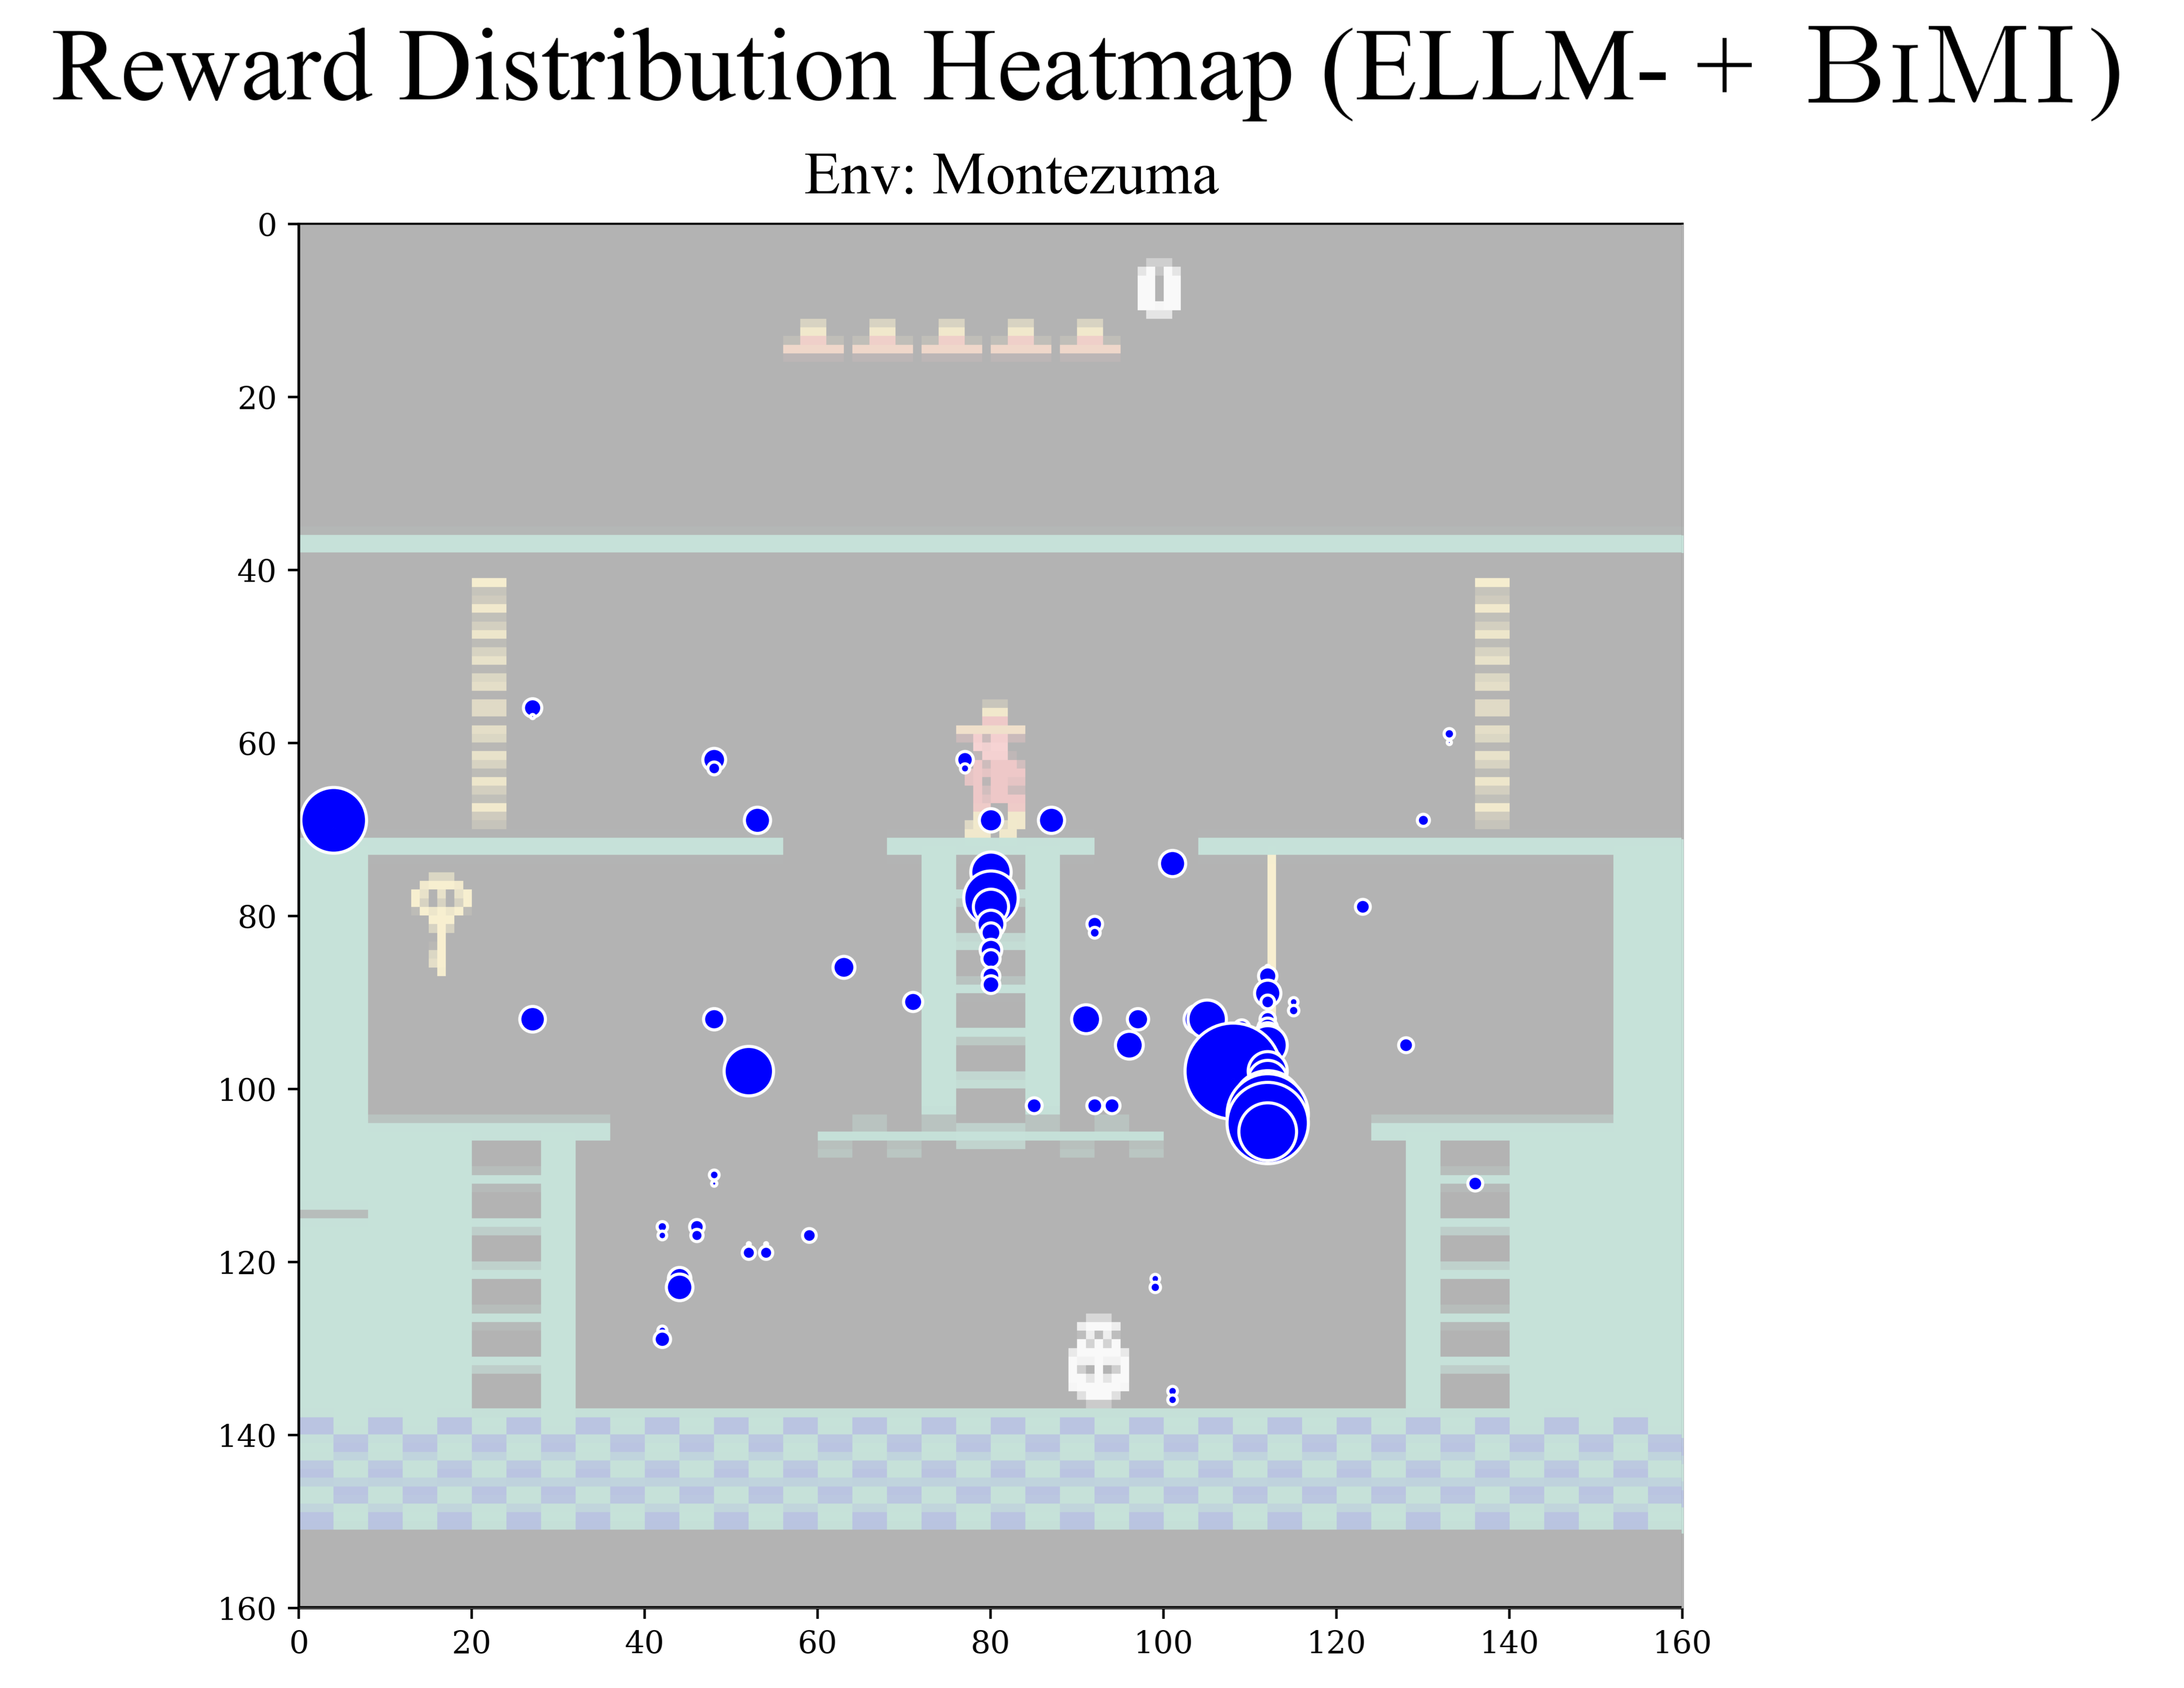
\includegraphics[width=\textwidth]{figures/Reward_Distribution_Heatmap_with_BIMI.png}
        \caption{The ratio of false positive rewards is significantly reduced after applying \textsc{BiMI}}
        \label{fig:reward_distribution_heatmap_with_bimi}
    \end{minipage}

\end{figure*}

\begin{wrapfigure}{r}{0.6\textwidth}
	\centering
    \caption{Score metric across environments (equivalent to total rewards, higher is better). $\star$ denotes baseline intrinsic reward model. VLM reward models without noise handling underperformed. All models are based on PPO.}
    \label{tab:stage_1_rl_results}
    \resizebox{0.6\columnwidth}{!}{%
    \begin{tabular}{lccccc}
    \hline
    Models        & Type          & \multicolumn{1}{c}{Monte.} & \multicolumn{1}{c}{Minigrid} & \multicolumn{1}{c}{Crafter} & \% vs. DEIR \\ \hline
    PPO           & Pure          & $0.151$             & $24.993$          & $16.863$          & $-28\%$              \\
    DEIR $\star$  & Intrinsic     & $0.174$             & $55.556$           & $19.758$          & --                   \\ \hline
    Pixl2R        & VLM & $0.142$             & $12.422$           & $9.409$           & $\mathbf{-49\%}$     \\
    ELLM-         & VLM & $0.150$             & $19.406$          & $10.826$          & $-41\%$              \\
    Pixl2R + DEIR & VLM + intr. & $0.176$             & $17.372$           & $10.440$          & $-38\%$              \\
    ELLM- + DEIR  & VLM + intr. & $0.178$             & $30.985$           & $11.857$          & $-27\%$             \\ \hline
    \end{tabular}%
    }
\end{wrapfigure}

\noindent\textbf{Prevalence of False Positives.} To address \textbf{H2}, we analyzed reward distribution heatmap from VLM-based reward models during training. The heatmap revealed a concerning trend: RL agents engage in reward hacking, receiving rewards across vast areas of the environment rather than just at goal states. For instance, in \emph{Montezuma} environment where the goal is to grab the key and escape the room, we observed that agents received rewards even for falling off cliffs, which undoubtedly contribute to the detrimental $\mathbb E [G^{\pi \in \Pi_B}]$ specified in Theorem~\ref{theo:convergence}. For environments without fixed camera views, we calculated the step offset between the current rewarded state and the actual goal state. A positive offset indicates that a reward was given before reaching the goal state, signifying a false positive reward, while a negative offset suggests that the agent reached the goal state but the reward model failed to recognize it, indicating a false negative reward (see Figure~\ref{fig:show_prevalence_of_noisy_rewards}). Interestingly, we observed a large amount of negative step offsets in Minigrid environments. We attribute this to Minigrid's abstract shape-based visual representations, which fall outside the VLM's pretraining distribution.


\noindent\textbf{Impact on Learning.}\quad We trained agents using learned VLM reward models and compared their learning efficacy against intrinsic reward models. As shown in Table~\ref{tab:stage_1_rl_results}, our results confirmed \textbf{H3}: \textit{instruction-guided RL agents using learned VLM reward models without noise handling consistently underperform compared to DEIR, the intrinsic reward-based RL agent.} To investigate the impact of false negatives versus false positives (\textbf{H4}), we designed an oracle Pixl2R model with two variants: a false negative model and a false positive model. The false negative model only rewards the agent for reaching subgoal states described in the instruction, with a probability of x\% that some rewarding states in the map are removed. In contrast, the false positive model rewards the agent for reaching every subgoal, but also introduces a 0.1 one-off reward for certain locations, covering x\% of the map. The results indicate that false negatives may be less detrimental to agent performance than false positives (see Figure~\ref{fig:FP_FN_comparison}). This performance difference can be explained through our theoretical framework: \quad (1) False negative models maintain the coefficient $\mathbb{E}[G^{\pi \in \Pi_G}] - \mathbb{E}[G^{\pi \in \Pi_B}]$, ensuring steady gradient ascent towards maximizing $P(\pi \in \Pi_G)$;
\quad (2) By decreasing $\mathbb{E}[G^{\pi \in \Pi_B}]$, false negative models minimize deviations from the target direction, leading to more stable learning.

In contrast, scenarios with high $\mathbb{E}[G^{\pi \in \Pi_B}]$ (i.e., the false positive case) significantly reduce the gradient ascent rate and also introduce deviations from the target direction. \textbf{These findings challenge the belief that false negatives are RL degeneracy's main problem \citep{du2023guiding}. This insight motivates our proposed solution, which focuses on reducing false positive rewards, accepting a slight increase in false negatives as a trade-off.} 




\section{Solution to the Reward Noise Issue}
\subsection{Binary Signal and Conformal Prediction Thresholding}
\label{sec:preferring-binary-signal}
Our experiments have shown that the issue of false positives may be more detrimental to learning than false negatives. Based on these findings, we we propose a reward function that provides one-time binary rewards only when the similarity between the agent's current trajectory and the instruction exceeds a high confidence threshold. This method effectively reduces the likelihood of rewarding unacceptable trajectories.
To achieve this, we introduce a thresholding mechanism using a calibration set of true positive trajectory-instruction pairs. This threshold, denoted as $\hat q$, is set to the empirical quantile of cosine similarity scores at the significance level $1 - \alpha$. Pairs whose similarity scores fall below this threshold $\hat q$ receive no reward. Conversely, pairs exceeding $\hat q$ receive a one-time $+1$ reward, i.e., $r^v_{\textsc{Bi}}(\tau, l_k) = \mathbf{1}_{\{p(l_k\mid \tau) \geq \hat q\}}$. This approach statistically guarantees a high probability (at least $1 - \alpha$) that true positive pairs are recognized while minimizing frequency of false positives errors \citep{sadinle2019least}. See Appendix~\ref{sec:pseudo-code-for-threshold} for detailed threshold calculation. 


\subsection{Mutual Information Maximization}
Intuitively, when we observe rewards coming from a particular signal source too frequently, we tend to downplay the significance of that signal to avoid over-reliance. This intuition is effectively captured by incorporating a \emph{mutual information maximization} term into the reward function. Specifically, the updated reward function $r^v_{\textsc{MI}}(\tau, l_k)$ measures the mutual information between the agent's trajectory and the instruction. Mathematically, it can be expressed as:
\begin{flalign}
    r^v_{\textsc{MI}}(\tau, l_k) & = I(l_k; \tau) = D_{KL}(p(l_k, \tau) \mid\mid p(l_k)p(\tau))\nonumber \\
                & = \mathbb E_{ \tau \sim \pi_{\theta}, l_k \sim L}[\log p (l_k \mid \tau) - \log p(l_k)]
\end{flalign}
\noindent where $p(l_k\mid \tau)$ comes from the similarity score provided by VLMs, and $p(l_k)$ is the frequency of the instruction $l_k$ being fulfilled by the agent's trajectory. Therefore, the second term in the equation serves as a regularization term that downplays the significance of the reward signal when it is too frequent. For instance, if a VLM frequently detects that the agent's actions are fulfilling the ``climbing the ladder'' instruction, even when the agent is performing unrelated tasks, the reward signal for this instruction will be downplayed. $p(l_k)$ is calculated as follows:
\begin{equation}
    p(l_k) = \mathbb E_{\tau \sim \pi_{\theta_{-1}}} \left[ \frac{\sum_{t=1}^{T_\tau}\mathbf{1}_{\{p(l_k\mid \tau_t) \geq \hat q \}}}{T_\tau} \right]
\end{equation}
\noindent Here, $\tau_t$ is the agent's trajectory up to time $t$, and if the VLM deems the trajectory as fulfilling the instruction (i.e., $p(l_k\mid \tau_t) \geq \hat q$), we increment the count. Dividing the count by the total trajectory length $T_\tau$ gives the empirical frequency of the instruction being fulfilled. The subscript $\theta_{-1}$ in $\pi_{\theta_{-1}}$ indicates that the trajectories are sourced from rollouts in the previous policy iteration, acknowledging the impracticality of real-time computation of $p(l_k)$ during an ongoing episode.

To enhance the stability of the training process, we adopt a linearized version of the mutual information maximization approach, as proposed by \citet{li2023internally}. Overall, \textsc{BiMI}, the proposed reward function that enhances the noise resilience of VLM-based reward models, can be expressed as follows:
\begin{equation}
    r^v_{\textsc{BiMI}}(\tau, l_k) = \max(\mathbf{1}_{\{p(l_k\mid \tau) \geq \hat q\}} - p(l_k),0)
\end{equation}
\noindent It's important to note that the \textsc{BiMI} approach primarily mitigates false positives (FP) rather than false negatives (FN). By implementing a high confidence threshold and a binary reward signal, we effectively reduce the likelihood of rewarding incorrect trajectories, thus addressing the FP issue. While this conservative approach may potentially increase FNs, as some correct trajectories might fall below the threshold, our experiments indicate that this trade-off is beneficial. We found that false positives are more detrimental to learning in instruction-guided RL tasks, justifying our preference for a method that prioritizes FP reduction. 


\section{Experiments}
\label{sec:experiments}


We evaluate the \textsc{BiMI} reward function using baseline agents (\emph{Pixl2R} and \emph{ELLM-}) and their \textsc{BiMI}-enhanced counterparts, while also exploring potential synergies with the intrinsic reward model DEIR. We follow the same experimental setup as in Section~\ref{sec:experiments_on_existence}, with additional details in Appendix~\ref{sec:experiments_stage_2_details}. 

\begin{figure*}[h]
    \centering
\begin{minipage}{0.6\textwidth}
        \captionof{table}{Model score across various environments. $\star$ is the baseline agents with a learned VLM-based reward model to compare with. \textsc{BiMI} significantly improves performance in \emph{Montezuma} and \emph{Minigrid}, while showing mixed results in \emph{Crafter} due to task-specific characteristics}
        \label{tab:stage_2_rl_performance}
        \resizebox{\columnwidth}{!}{%
\begin{tabular}{@{}llclclc@{}}
\toprule
Methods              & \multicolumn{1}{c}{Montezuma} & \% vs. $\star$ & \multicolumn{1}{c}{Minigrid} & \% vs. $\star$ & \multicolumn{1}{c}{Crafter} & \% vs. $\star$ \\ \midrule
Pixl2R $\star$       & $0.142 \pm 0.003$             & --                   & $12.422 \pm 2.439$           & --                   & $9.409 \pm 0.022$           & --                   \\
Pixl2R + Bi          & $0.137 \pm 0.009$             & $-3.5\%$             & $31.236 \pm 2.040$           & $151\%$              & $10.735 \pm 0.784$          & $14\%$               \\
Pixl2R + BiMI        & $0.162 \pm 0.022$             & $14\%$               & $37.507 \pm 7.832$           & $199\%$              & $7.951 \pm 0.351$           & $-15\%$              \\ \midrule
Pixl2R + DEIR        & $0.176 \pm 0.009$             & $23\%$               & $17.372 \pm 0.514$           & $39\%$               & $10.440 \pm 1.015$          & $10\%$               \\
Pixl2R + BiMI + DEIR & $0.267 \pm 0.016$             & $88\%$               & $57.759 \pm 2.157$           & $364\%$              & $11.014 \pm 0.190$          & $17\%$               \\ \midrule
ELLM- $\star$        & $0.150 \pm 0.004$             & --                   & $19.406 \pm 10.067$          & --                   & $10.826 \pm 1.017$          & --                   \\
ELLM- + Bi           & $0.151 \pm 0.016$             & $0.6\%$              & $29.788 \pm 1.290$           & $53\%$               & $11.175 \pm 0.601$          & $3.2\%$              \\
ELLM- + BiMI         & $0.156 \pm 0.014$             & $4.0\%$              & $33.683 \pm 3.990$           & $74\%$               & $9.425 \pm 0.267$           & $-12\%$              \\ \midrule
ELLM + DEIR          & $0.178 \pm 0.029$             & $20\%$               & $30.985 \pm 3.507$           & $59\%$               & $11.857 \pm 1.152$          & $9.5\%$               \\
ELLM- + BiMI + DEIR  & $0.279 \pm 0.078$             & $86\%$               & $56.281 \pm 6.193$           & $190\%$              & $13.170 \pm 0.393$          & $22\%$               \\ \bottomrule
\end{tabular}%
}
    
\end{minipage}
\hspace{0.1cm}
\begin{minipage}{0.345\textwidth}
    \centering
    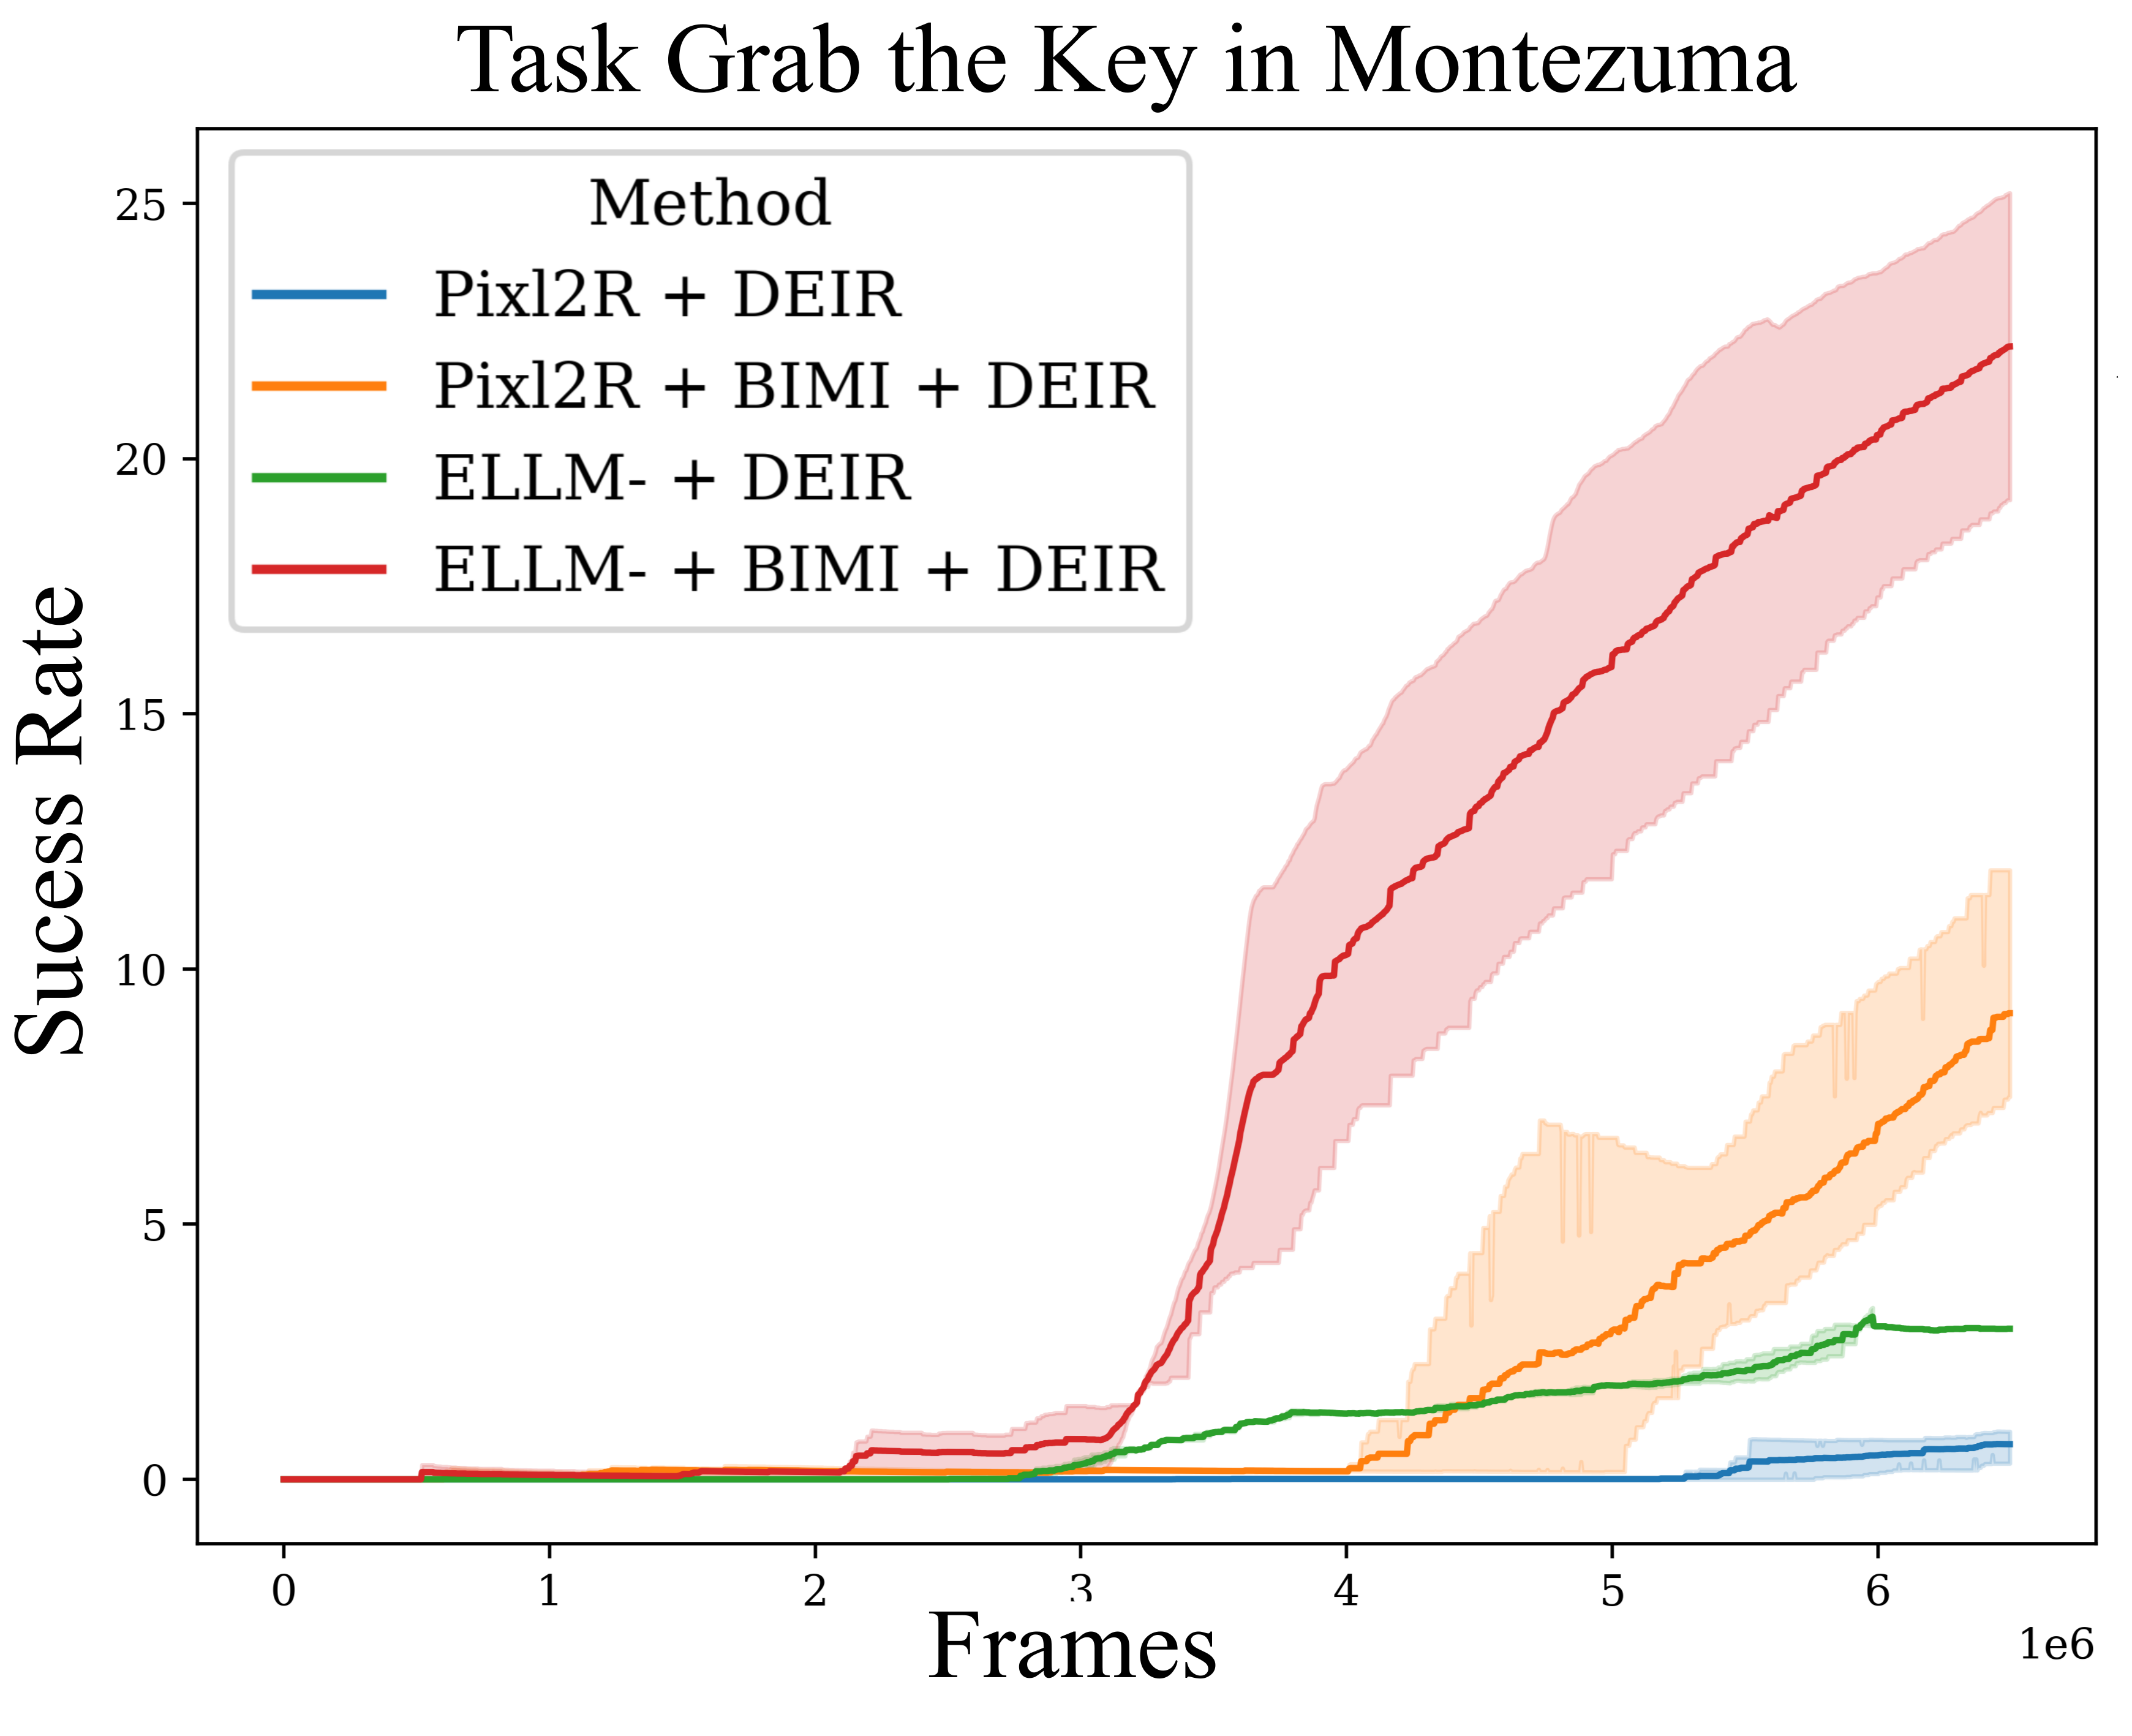
\includegraphics[width=\linewidth]{figures/montezuma_difficult_task_success_rate.png}
    \caption{\textsc{BiMI} reward showed faster and higher success rates on difficult tasks in Montezuma} 
    \label{fig:montezuma_difficult_task_success_rate}
\end{minipage}
\end{figure*}



\subsection{Overall Performance and Ablation Study}
\label{subsec:ablation}
The overall improvements were substantial. As shown in Table~\ref{tab:stage_2_rl_performance}, \textsc{BiMI} led to a 67\% improvement for \emph{Pixl2R} and a 22\% improvement for \emph{ELLM-}. These results are also illustrated in Figure~\ref{fig:montezuma_difficult_task_success_rate} Figure~\ref{fig:main_result_lineplot_score} in Appendix~\ref{app_subsec:detailed_bimi_exp_result}.
Our ablation study highlights the distinct contributions of the binary reward (\textsc{Bi}) and Mutual Information (\textsc{MI}) components within the \textsc{BiMI} framework. The binary reward mechanism alone accounted for a substantial 36.5\% improvement in performance. When excluding the results from \emph{Crafter}, \textsc{MI} component further contributes a 23\% improvement over the binary reward alone.  Please see Appendix~\ref{app_subsec:detailed_bimi_exp_result} for result details for each test environment.

\section{Conclusion}
Our research reveals two key findings in agent learning using VLM-based reward models: (1) false positive rewards, rather than false negatives, are more detrimental to policy learning; and (2) our proposed \textsc{BiMI} reward function significantly mitigates the slowdown in learning caused by false positives, thereby paving the way for more reliable and effective ``language as an interface'' RL systems in practical settings.

\noindent\textbf{Limitation.}\quad Our study primarily focused on linear sequences of language instructions, excluding more complex cases. Future research should investigate conditional and ambiguous instructions, which likely introduce additional challenges for VLM-based reward models. We also did not explore finetuning the VLM during agent training, a useful strategy as discussed by \citet{fufurl2024}.


% no \bibliographystyle is required, since the corl style is automatically used.
\bibliography{example}  % .bib
\pagebreak
\appendix
\section{Technical Appendix}
Continued from the main text of \emph{Overcoming Reward Model Noise in Instruction-Guided Reinforcement Learning}, the technical appendix consist of the following: 
\begin{itemize}
    \item \textbf{\S \ref{app_subsec:property_of_sparse_reward} Property of Sparse Reward Function}, which discuss why sparse reward function results in the categorization of policies into a set of acceptable policies and a set of unacceptable policies but not others.
    \item \textbf{\S \ref{sec:proofofreductionofconvergence} Proof of the Reduction of Convergence Rate}, which is referred in Section~\ref{sec:background}.
    \item \textbf{\S \ref{sec:implementation_details_first_stage} Implementation Details of the Experiments}, which specify the implementation details for both the first and second stage experiments in Section~\ref{sec:experiments_on_existence} and Section~\ref{sec:experiments} respectively.
    \item \textbf{\S \ref{sec:experiments_stage_1_details} Additional Details of the Experiments of False Positive Rewards}, which is referred in Section~\ref{sec:experiments_on_existence}.
    \item \textbf{\S \ref{sec:pseudo-code-for-threshold} Pseudo-code for Empirical Quantile Calculation for Binary Signal Threshold}, which is referred in Section~\ref{sec:preferring-binary-signal}.
    \item \textbf{\S \ref{sec:experiments_stage_2_details} Additional Implementation Details of the Experiments of \textsc{BiMI} Reward Function}, which is referred in Section~\ref{sec:experiments}.
    \item \textbf{\S \ref{app_subsec:detailed_bimi_exp_result} Detailed Experiment Results of \textsc{BiMI} Reward Function}, which provides detailed experiment results of \textsc{BiMI} reward function, which is referred in Section~\ref{sec:experiments}.
\end{itemize}

\subsection{Sparse Reward Function and Range-SOAP}
\label{app_subsec:property_of_sparse_reward}

Formally, \citet{Abel2021OnTE} defined that: 

\begin{theorem}[\citet{Abel2021OnTE}]
\label{theo:sparse_reward_range_soap}
A reward function realizes a Range Set of Acceptable Policies (Range-SOAP) $\Pi_G$ when there exists an $\epsilon \geq 0$ such that every $\pi_g \in \Pi_G$ is $\epsilon$-optimal in start-state value, $V^*(s_0) - V^{\pi_g}(s_0) \leq \epsilon$, while all other policies are worse. 
\end{theorem}

When the reward signal is sparse, the agent only receives a reward upon reaching some goal states, and the reward function does not provide any feedback during the intermediate steps. We argue that the sparse reward function realizes a Range-SOAP, leading to the categorization of policies into acceptable and unacceptable policies.

\begin{proposition}
    Sparse reward function ``realizes'' Range-SOAP (i.e., Range Set of Acceptable Policies). 
\end{proposition}


\noindent\textbf{Justification:}

A sparse reward function, where the agent only receives a reward upon completing the task, cannot prefer policies that lead to shorter task completion times. This is because either the agent completes the goal very quickly or slowly, they will receive nearly the same amount of cumulative rewards, and the reward function will not show a strong preference. 

Since the sparse reward function does not induce a strict partial ordering on the policies, we say this reward function cannot realize a Partial Ordering (PO) task. Specifically, a PO on policies is a generalization of a Set of Acceptable Policies (SOAP) task. In a PO, the agent specifies a partial ordering on the policy space, where some policies are identified as ``great'', some as ``good'', and some as ``bad'' to strictly avoid, while remaining indifferent to the rest. 

Therefore, the sparse reward function can realize a Set of Acceptable Policies (SOAP), where there is a set of policies that are all considered ``good'' or near-optimal, while all other policies are worse. 

Furthermore, the sparse reward function will lead to a Range-SOAP, rather than an Equal-SOAP. Specifically, Equal-SOAP is a SOAP where all the acceptable policies are equally optimal in start-state value. This is because the good policies in the SOAP may differ slightly in their start-state values, as some may reach multiple goal states in the environment and thereby receiving different cumulative rewards. Therefore, the sparse reward function will realize a Range-SOAP, where there is a range of acceptable policies that are all near-optimal in start-state value.


\subsection{Proof of the Reduction of Convergence Rate}
\label{sec:proofofreductionofconvergence}

Specifically, the update rule of Actor-Critic algorithm is: 

\begin{itemize}
    \item \textbf{Critic}: 
    \begin{equation}
        \phi \leftarrow \phi - \alpha_\phi \nabla_\phi (\delta)^2
    \end{equation}
    where 
    \begin{description}
        \item $\delta = \mathbb E_{\pi_{\theta}}[G^{\pi_{\theta}} - Q_\phi (s,a)]$ is the Monte Carlo (MC) estimation error, $Q_\phi (s,a)$ is the $Q$-value function which measures the expected discounted cumulative reward given the state $s$ and action $a$, and $\pi_{\theta}$ is the policy.
        \item $G^{\pi_{\theta}}$ is the rollout cumulative rewards from the trajectory $\tau^{\pi_{\theta}}$ generated from $\pi_{\theta}$.
    \end{description}
    \item \textbf{Actor}: 
    \begin{equation}
        \theta \leftarrow \theta + \alpha_\theta \frac{Q_\phi(s,a) \nabla_\theta \pi_\theta(a|s)} {\pi_\theta(a|s)}
    \end{equation}
\end{itemize}

% For the sake of brevity, we denote $G^\pi(s_t,a_t) = \sum_{l=0}^{\infty} \gamma^l R(s_{t+l},a_{t+l})$ where $\tau^\pi = (s_0, a_0, s_1, a_1, s_2, ...)$ and $G^\pi = G^\pi(s_0,a_0)$, which is the cumulative discounted reward for $\tau^\pi$. 
We need to make the following assumptions to simplify the theoretical analysis: 

\begin{enumerate}
    \item We use $\Pi_G$ to represent the set of acceptable policies and use $\Pi_B$ as an arbitrary set of ``not acceptable'' policies that are learned to follow instruction but fail to reach subgoals, i.e., $\Pi_{B} \cap \Pi_{G} = \varnothing$.

    \item Assume the policy class parameterized by $\theta$ should be expressive enough to capture optimal or near-optimal policies, and the policy is initialized randomly from uniform distribution, i.e., $\pi_{\theta_{0}} \sim \mathcal U(\Pi)$. Meanwhile, the Q-value is initialized as $Q_{\phi_{0}}(s, a) = 0, \forall_{s\in S} \forall_{a\in A}$.

    \item We assume that $|\Pi_{G}|$ and $|\Pi_B|$ is a fixed number predefined by the task environment while $\mathbb E[G^\pi| \pi \in \Pi_{B}]$ is non-zero as false positive rewards are unavoidable in real-world VLMs.
\end{enumerate}

Since the update rule for $Q$-value is a gradient descent on $\| \mathbb E [G^{\pi_\theta} - Q_\phi(s,a)] \|^2$ and also we have that $\{\Pi_{B}, \Pi_{G}, \Pi \setminus (\Pi_{B} \cup \Pi_{G})\}$ is a countable partition of the policy universe $\Pi$, the updated $Q$-value will approach as follows:
\begin{flalign}
   &&             & \quad Q_\phi(s,a) \rightarrow \mathbb E [G^{\pi_\theta}] && \nonumber \\ 
   &&             &=          P(\pi_\theta \in \Pi_{B}) \cdot \mathbb E [G^{\pi_\theta} | \pi_\theta \in \Pi_{B}] \nonumber \\
   &&             &\qquad +  P(\pi_\theta \in \Pi_{G}) \cdot \mathbb E [G^{\pi_\theta} | \pi_\theta \in \Pi_{G}] \nonumber \\
   &&             &\qquad + P(\pi_\theta \in \Pi \setminus (\Pi_{B} \cup \Pi_{G}) ) \nonumber \\
   &&             &\qquad \cdot \mathbb E [G^{\pi_\theta} | \pi_\theta \in \Pi \setminus (\Pi_{B} \cup \Pi_{G})]     && \nonumber \\
   &&             &=          P(\pi_\theta \in \Pi_{B}) \cdot \mathbb E [G^{\pi_\theta} | \pi_\theta \in \Pi_{B}]  \nonumber \\
   &&             &\qquad +  P(\pi_\theta \in \Pi_{G}) \cdot \mathbb E [G^{\pi_\theta} | \pi_\theta \in \Pi_{G}]
\end{flalign}
Given that the update rule for policy $\pi$ is the gradient ascent on $Q_\phi(s,a)\pi_\theta(a|s)$, we have the following:
\begin{flalign}
    &&              &\quad     \nabla_\theta Q_\phi(s,a)\pi_\theta(a|s)          &&  \nonumber \\
    &&                                          &= (\nabla_\theta P(\pi_{\theta_{old}} \in \Pi_{B}) \cdot \mathbb E [G^{\pi_{\theta_{old}}} | \pi_{\theta_{old}} \in \Pi_{B}] \pi_\theta(a|s)) && \nonumber \\
    &&                                          &\qquad + (\nabla_\theta P(\pi_{\theta_{old}} \in \Pi_{G}) \nonumber \\
    &&                                          &\qquad \cdot \mathbb E [G^{\pi_{\theta_{old}}} | \pi_{\theta_{old}} \in \Pi_{G}] \pi_\theta(a|s)) && \nonumber \\
    &&                                          &= P(\Pi_{B}) \cdot \mathbb E [G^{\Pi_{B}}] \nabla_\theta \pi_\theta(a|s) \nonumber\\
    &&                                          &\qquad + P(\pi_{G}) \cdot \mathbb E [G^{\pi_{G}}] \nabla_\theta \pi_\theta(a|s) &&  \nonumber \\
    &&                                          &= (1 - P(\pi_{G}) - P(\pi_\theta \in \Pi \setminus (\Pi_{B} \cup \Pi_{G}) )) \nonumber \\
    &&                                          &\qquad \cdot \mathbb E [G^{\Pi_{B}}] \nabla_\theta \pi_\theta(a|s) + P(\pi_{G}) \cdot \mathbb E [G^{\pi_{G}}] \nabla_\theta \pi_\theta(a|s) && \nonumber \\
    &&                                          &= \textit{const} \cdot \mathbb E [G^{\Pi_B}] \nabla_\theta \pi_\theta(a|s) \nonumber\\
    &&                                          &\qquad + ( \mathbb E [G^{\pi_G}] - \mathbb E [G^{\Pi_B}]) P(\pi_G) \nabla_\theta \pi_\theta(a|s)
\end{flalign}   

\noindent {Justification of the assumptions.}
\begin{itemize}
    \item Regarding the non-zero probability of recovering the optimal policy at initialization, it is standard in theoretical analyses to assume a uniform distribution of a random variable at initialization (see \citet{agarwal2021theory}). This assumption does not contradict the conclusion about the convergence rate deterioration in Theorem~\ref{theo:convergence}.
    \item In reference to the realizability condition implied by Assumption 2, the expressiveness of the policy class parameterized by $\theta$ is an underlying assumption for deep learning models, supported by the The Universal Approximation Theorem \citep{hornik1989multilayer}. 
\end{itemize}
\noindent \textbf{Observation.} Since the goal of the learning agent is to maximize $P(\pi \in \Pi_G)$ (i.e., to converge to an acceptable policy), we can see that the second term provides the target direction with rate $( \mathbb E [G^{\pi \in \Pi_G}] - \mathbb E [G^{\pi \in \Pi_B}])$. Therefore, the ascent rate will decrease when the cumulative rewards from trajectories that cannot reach the goal state (i.e., the false positive rewards) gets higher. Moreover, the first term $\textit{const} \cdot \mathbb E [G^{\Pi_B}] \nabla_\theta \pi_\theta(a|s)$ can be regarded as the deviation of target direction. It shows that the level of deviation is also positively proportional to the magnitude of rewards coming from failed trajectories. This theorem follows the intuition that the presence of false positive rewards can slow down the convergence rate of the learning agent.

\subsection{Implementation Details of the Experiments}
\label{sec:implementation_details_first_stage}
\subsubsection{Environment Details}
We describe each testing environment used in our experiments. More details introduction can be found in on the official project homepage of each benchmark \citep{chevalier2018babyai, Bellemare2012TheAL, Hafner2021BenchmarkingTS}. 
\begin{itemize}
    \item \textbf{Crafter} features randomly generated 2D worlds where the player needs to forage for food and water, find shelter to sleep, defend against monsters, collect materials, and build tools. The original Crafter environment does not have a clear goal trajectory or instructions; agents are aimed at surviving as long as possible and exploring the environment to unlock new crafting recipes. We modified the environment to include a preset linear sequence of instructions to guide the agent to mine diamond. However, this instruction was found to hinder the agent's performance. The nature of the task requires dynamic strategies and real-time decision-making, but the fixed instructions limited the agent. For example, the instruction did not account for what to do when the agent is attacked by zombies.
    \item \textbf{Montezuma's Revenge} is a classic adventure platform game where the player must navigate through a series of rooms to collect treasures and keys. The game is known for its sparse rewards and challenging exploration requirements. We manually annotate 97 instructions for the agent to follow, guiding it to conquer the game. The instructions were designed to guide the agent through the game's key challenges, such as avoiding enemies, collecting keys, and unlocking doors.
    \item \textbf{Minigrid `Go to seq' Task}: We use the `Go to seq' task in the Minigrid environment, where the agent must navigate through a sequence of rooms and touch target objects in the correct order. This is a sparse reward task where the agent receives a reward of 1 only upon completing the entire sequence correctly. During the training phase, we randomly generate 50 different tasks, each with a room size of 5, 3 rows, and 3 columns. Each task features a unique room layout and target object sequence. The instruction complexity is set to 3, meaning there are at least 3 target objects to interact with in a specific order.
\end{itemize}

\begin{figure}[H]
    \centering
    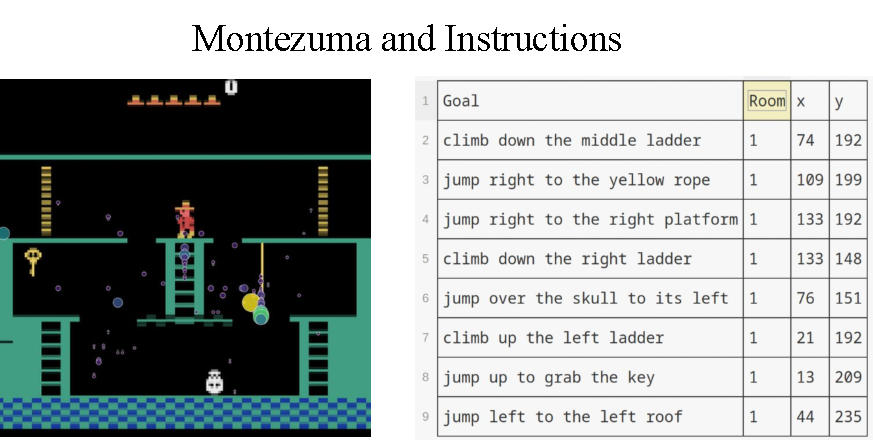
\includegraphics[width=0.63\columnwidth]{appendix_figures/montezuma_task_illu.pdf}
    \caption{Illustration of the Montezuma's Revenge task. The agent must navigate through a series of rooms to collect treasures and keys.}
\end{figure}

\begin{figure}[H]
    \centering
    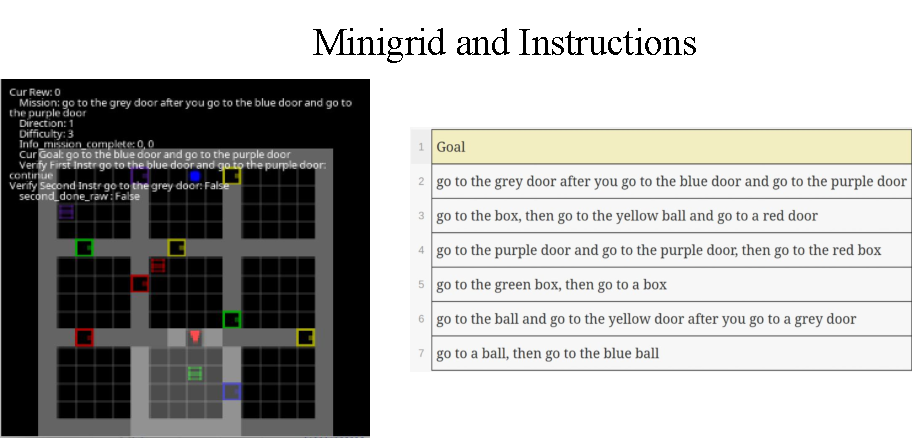
\includegraphics[width=0.7\columnwidth]{appendix_figures/minigrid_task_illu.pdf}
    \caption{Illustration of the Minigrid `Go to seq' task. The agent must navigate through a sequence of rooms and touch target objects in the correct order.}
\end{figure}

\begin{figure}[H]
    \centering
    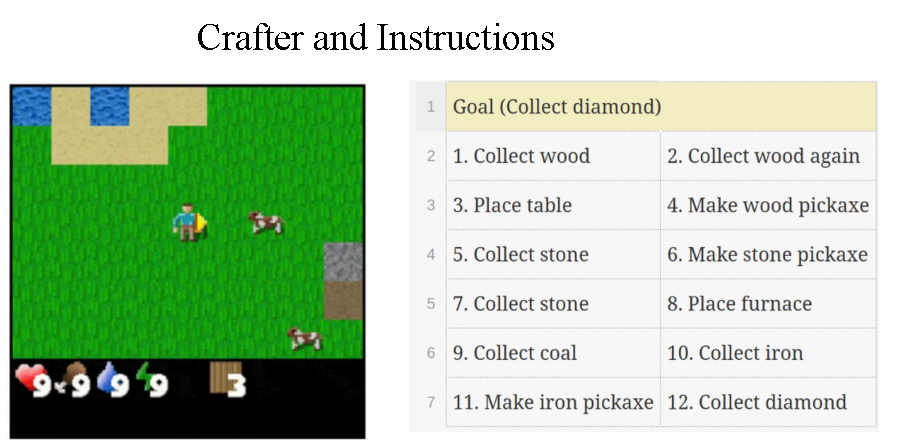
\includegraphics[width=0.67\columnwidth]{appendix_figures/crafter_task_illu.pdf}
    \caption{Illustration of the Crafter task. The agent must survive as long as possible and explore for new crafting recipes.}
\end{figure}

\subsubsection{Instruction-Guide Procedure Details}
The VLM-based reward model will have a pointer to the sequence of the instruction sentence, starting at the first sentence. For original models \emph{Pixl2R} and \emph{ELLM-}, we follow the setting in there original work where for each instruction sentence (yes, the full instruction essay will be split into multiple sentences and treat each sentence as atomic instruction $l_k$), the reward model will have a maximum cap of rewards (2.0) it can assign to the agent in one episode. When the cap is reached, the reward model will move its pointer to the next instruction sentence. For the \textsc{BiMI} reward model, the reward model will move its pointer to the next instruction sentence when the binary signal is triggered. 

\subsubsection{Finetuning VLM-based Reward Models}
In contrast to previous work on Instruction-guided RL where they rely on hand-crafted oracle multimodal reward models, we use actual pretrained VLMs to generate reward signals. 2 VLM backbone models are used in our experiments: 1) \emph{CLIP} \citep{Radford2021LearningTV}, pretrained by image-text pairs; and (2) \emph{X-CLIP} \citep{Ma2022XCLIPEM}, pretrained by video-text pairs. In particular, \emph{Pixl2R} uses \emph{CLIP} because it only uses the single latest frame as input. In contrast, \emph{ELLM-} takes a slice of trajectory (i.e., multiple frames) as input, and thus uses either \emph{X-CLIP} or \emph{CLIP} with additional RNN encoder as the reward model.

Due to the cartoonish and abstract visuals of the testing environments, we need to further fine-tune the VLMs to adapt to this new visual domain. We use well-trained expert agents based on \citet{moon2023ad} to generate expert trajectories for the Crafter environments and annotate them with instructions using internal information from the game engine. For Minigrid environments, we use classical search-based planning robots to generate expert trajectories and annotate them with the corresponding task instructions. For Montezuma's Revenge, we manually annotate the expert trajectories.

For Minigrid and Crafter, we have 80,000 training pairs, while for Montezuma's Revenge, we have around 300 training pairs. These training data are of high quality, as we have made every effort to avoid false positive rewards due to poor training data quality. \textbf{To enhance our models' robustness, we also employed contrastive learning techniques during VLM training, utilizing similar manipulated data as hard negatives.} However, despite the fine-tuning process, false positive rewards remain unavoidable.

\begin{figure}[H]
    \centering
    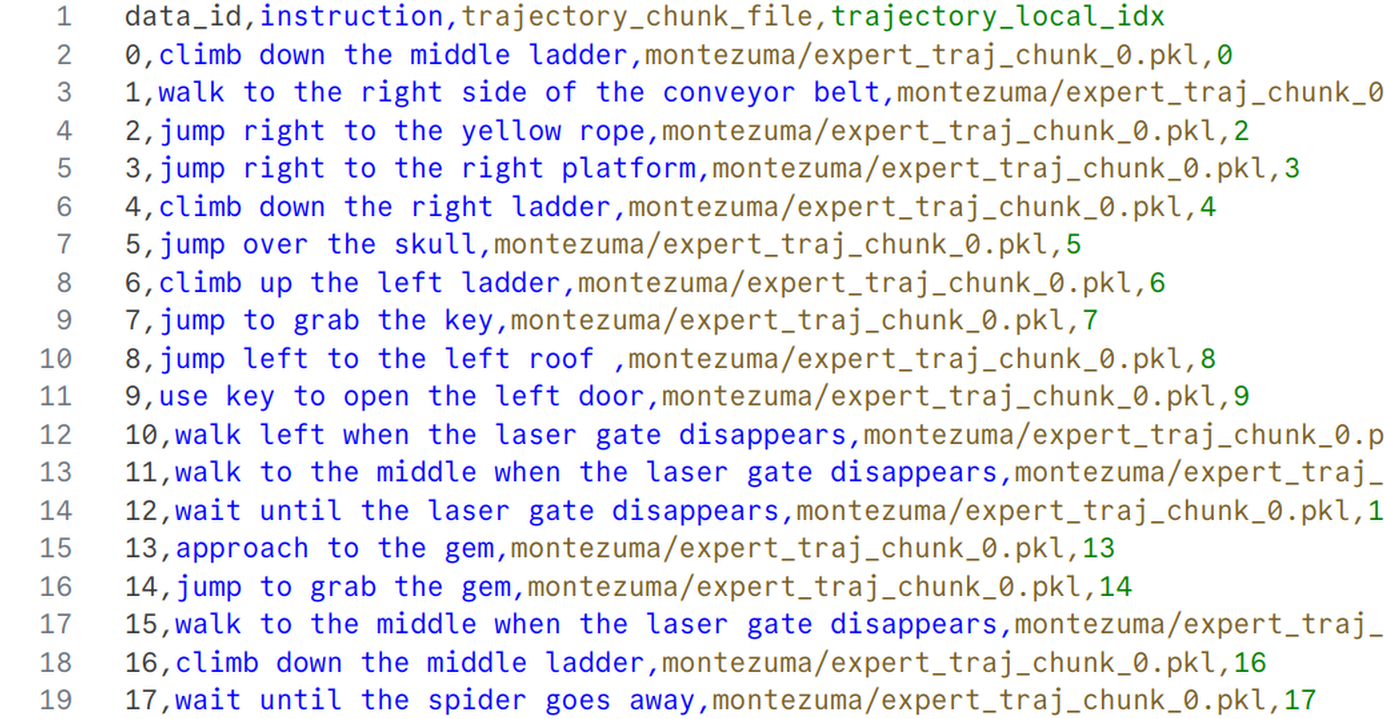
\includegraphics[width=\columnwidth]{appendix_figures/training_data_example.png}
    \caption{Example of training data for the Montezuma environment.}
\end{figure}

We used the threshold $\hat q$ introduced in Section~\ref{sec:preferring-binary-signal} to make binary classification on the testing pairs to evaluate the performance of the fine-tuned VLM-based reward models. We found that VLM models had difficulty achieving high accuracy on Minigrid environment, which is likely due to the too abstract and cartoonish nature of the environment, causing the VLMs to struggle to learn the visual-textual correspondence. We also found that X-CLIP did not perform better than CLIP in our experiments. We hypothesize that the cartoonish nature of the testing environments may have caused the X-CLIP model to struggle to learn the visual-textual correspondence. Thus, we used CLIP as the backbone model throughout our following experiments. The performance of the fine-tuned VLM-based reward models is shown in Table~\ref{tab:vlm_performance}. \textbf{Even when the precision score reaches 0.98, indicating that only 2\% of the rewards are false positives in the validation set, the agent can still significantly underperform in the testing environments. The core issue is that in out-of-distribution (O.O.D.) testing environments, false positive rewards are prevalent and inevitable. Therefore, it is crucial to design a reward function that is robust to reward noise.}

\begin{table}[H]
    \centering
    \caption{Performance of fine-tuned VLM reward model on the testing dataset using the 90th percentile empirical quantile as threshold}
    \label{tab:vlm_performance}
    \resizebox{0.7\columnwidth}{!}{%
    \begin{tabular}{@{}llllll@{}}
    \toprule
    Environment & Precision & Accuracy & F1 Score & Recall & Model       \\ \midrule
    Crafter     & 0.9847    & 0.9466   & 0.8538   & 0.9702 & CLIP ELLM-  \\
    Crafter     & 0.9799    & 0.9028   & 0.7618   & 0.9842 & CLIP Pixl2R \\
    Crafter     & 0.2095    & 0.2514   & 0.2868   & 0.9657 & XCLIP ELLM- \\ \midrule
    Minigrid    & 0.7260    & 0.9200   & 0.7849   & 0.9763 & CLIP ELLM-  \\
    Minigrid    & 0.6992    & 0.9086   & 0.7592   & 0.9616 & CLIP Pixl2R \\
    Minigrid    & 0.1716    & 0.2310   & 0.2642   & 0.9704 & XCLIP ELLM- \\ \midrule
    Montezuma   & 0.8838    & 0.9638   & 0.8825   & 0.9478 & CLIP ELLM-  \\
    Montezuma   & 0.8343    & 0.9108   & 0.7652   & 0.9842 & CLIP Pixl2R \\
    Montezuma   & 0.8044    & 0.9259   & 0.8045   & 0.9657 & XCLIP ELLM- \\ \bottomrule
    \end{tabular}%
    }
    \end{table}


\subsubsection{Hyperparameters for Instruction-Guided RL Agents}
In the experiments, all methods are implemented based on PPO with same model architecture. The Minigrid and Crafter environments use the same training hyperparameters as the Achievement Distillation paper \citep{moon2023ad}. For Montezuma's Revenge, we found that the performance of the agent was sensitive to the gamma and GAE lambda parameters. To improve the performance of agents in Montezuma's Revenge, we took two additional steps: (1) normalizing the observation inputs when computing the rewards, and (2) not normalizing the advantage during the GAE calculation. The hyperparameters are shown in the following tables.

\begin{figure}[H]
    \centering
\begin{minipage}{0.4\columnwidth}
    \centering
    \captionof{table}{Model Parameters}
    \label{tab:ppo_model_parameter}
    \resizebox{\linewidth}{!}{%
    \begin{tabular}{@{}ll@{}}
        \toprule
    Parameter                 & Value              \\ \midrule
    model\_cls                & ``PPORNNModel''      \\
    hidsize                   & 1024               \\
    gru\_layers               & 1                  \\
    impala\_kwargs            &                    \\
    - chans                   & {[}64, 128, 128{]} \\
    - outsize                 & 256                \\
    - nblock                  & 2                  \\
    - post\_pool\_groups      & 1                  \\
    - init\_norm\_kwargs      &                    \\
    - batch\_norm             & false              \\
    - group\_norm\_groups     & 1                  \\
    dense\_init\_norm\_kwargs &                    \\
    - layer\_norm             & true              \\ \bottomrule
    \end{tabular}%
    }
\end{minipage}
\hspace{0.5cm}


\end{figure}
\begin{figure}[H]
    \centering
\begin{minipage}{0.35\columnwidth}
    \centering
    \captionof{table}{Crafter and Minigrid RL Parameters}
    \label{tab:crafter_minigrid_rl_parameter}
    \resizebox{\linewidth}{!}{%
    \begin{tabular}{@{}ll@{}}
        \toprule
    Parameter         & Value          \\ \midrule
    gamma              & 0.95  \\
    gae\_lambda        & 0.65  \\
    algorithm\_cls    & ``PPOAlgorithm'' \\
    algorithm\_kwargs &                \\
    - ppo\_nepoch     & 3              \\
    - ppo\_nbatch     & 8              \\
    - clip\_param     & 0.2            \\
    - vf\_loss\_coef  & 0.5            \\
    - ent\_coef       & 0.01           \\
    - lr              & 3.0e-4         \\
    - max\_grad\_norm & 0.5            \\
    - aux\_freq       & 8              \\
    - aux\_nepoch     & 6              \\
    - pi\_dist\_coef  & 1.0            \\
    - vf\_dist\_coef  & 1.0           \\ \bottomrule
    \end{tabular}%
    }
\end{minipage}
\end{figure}

\begin{table}[H]
    \centering
    \caption{Montezuma RL Training Parameters}
    \label{tab:monte_rl_params}
    \resizebox{0.35\columnwidth}{!}{%
    \begin{tabular}{@{}ll@{}}
    \toprule
    Parameter             & Value          \\ \midrule
    gamma                 & 0.99           \\
    gae\_lambda           & 0.95           \\
    int\_rew\_type        & ``rnd''          \\
    pre\_obs\_norm\_steps & 50             \\
    algorithm\_cls        & ``PPOAlgorithm'' \\
    algorithm\_kwargs     &                \\
    - update\_proportion  & 0.25           \\
    - ppo\_nepoch         & 3              \\
    - ppo\_batch\_size    & 256            \\
    - clip\_param         & 0.1            \\
    - vf\_loss\_coef      & 0.5            \\
    - ent\_coef           & 0.001          \\
    - lr                  & 1.0e-4        \\ \bottomrule
    \end{tabular}%
    }
    \end{table}

\subsection{Additional Details of the Experiments on the Impact of Noisy Rewards}
\label{sec:experiments_stage_1_details}

\noindent\textbf{Evaluation Metric Details}\quad
In our experiments, we used a score metric adapted from the Crafter paper to evaluate agent performance across different environments. This score metric aggregates success rates for individual subtasks using a geometric mean. This metric was chosen over the \emph{maximum total rewards} metric for several reasons:
\begin{enumerate}
    \item \textbf{Consistency in Sparse Reward Settings:} Sparse reward environments often pose significant challenges for reinforcement learning agents. An agent might occasionally achieve high rewards by chance in one rollout but fail to replicate this success consistently in subsequent rollouts. This variability can lead to misleading evaluations if only the maximum total rewards are considered. The Score metric, by measuring the success rate of achieving each subgoal, provides a more stable and consistent measure of an agent's performance.
    \item \textbf{Capturing Learning Stability:} The Score metric evaluates the agent's ability to consistently reproduce successful behaviors across multiple episodes. This is crucial in sparse reward settings, where the agent's performance can fluctuate significantly. By focusing on the success rates of individual subtasks, the Score metric offers a more granular and reliable assessment of the agent's learning progress and stability.
    \item \textbf{Crafter Benchmark Standard:} The Crafter benchmark, which introduces the Score metric, is a well-regarded standard.
\end{enumerate}

Crafter codebase provides \emph{score} metric calculation by default. For Minigrid and Montezuma environments, we use the internal information from the game engine to detect whether the subtasks are completed, thus facilitating the calculation of the \emph{score} metric. 

\subsubsection{Details of Manipulated Trajectory-Instruction Pairs to Evaluate Robustness }
We evaluated the models' sensitivity by examining how cosine similarity scores change for manipulated trajectory-instruction pairs. These manipulations were designed to test the robustness of the models against various types of noise. Here's a detailed breakdown of the manipulations:

\begin{enumerate}
    \item \textbf{Trajectory Reversal:} We inverted the sequence of frames within each trajectory (i.e., \texttt{frames = frame[::-1]}) to assess the model's ability to detect reversed state transitions. This manipulation tests whether the model can distinguish between forward and backward progression in the state transition.
    \item \textbf{Instruction Negation:} We modified the original instructions by adding negation (e.g., changing ``do $l_k$'' to ``do not do $l_k$'' or ``avoid $l_k$''). This tests the model's sensitivity to semantic changes in the instruction that fundamentally alter the goal.

    \item \textbf{Instruction Rephrasing:} We rephrase the original instructions while maintaining their core meaning. This evaluates the model's robustness to linguistic variations and its ability to capture the essential semantic content of instructions.
    
    \item \textbf{Concatenation and Order Swapping:} Given two trajectory-instruction pairs $(\tau_1, l_1)$ and $(\tau_2, l_2)$, we created concatenated pairs and then swapped the order in one modality. For example:
        \begin{itemize}
            \item Original concatenation: $(\tau_1 + \tau_2, l_1 + l_2)$
            \item Swapped trajectory: $(\tau_2 + \tau_1, l_1 + l_2)$
            \item Swapped instruction: $(\tau_1 + \tau_2, l_2 + l_1)$
        \end{itemize}
        This tests the model's sensitivity to the order of components in multi-step tasks.
    
    \item \textbf{Concatenation with Partial Content:} We concatenated pairs but truncated one modality. For instance:
        \begin{itemize}
            \item Truncated trajectory: $(\tau_1, l_1 + l_2)$
            \item Truncated instruction: $(\tau_1 + \tau_2, l_1)$
        \end{itemize}
        This assesses the model's ability to detect partial mismatches in longer sequences.
    
\end{enumerate}

\subsection{Pseudo-code for Empirical Quantile Calculation for Binary Signal Threshold}
\label{sec:pseudo-code-for-threshold}

Using empirical quantile as threshold guarantees a high probability (at least $1 - \alpha$) that the true positive pairs are recognized while minimizing the average number of mistakes predicting false positives \citep{sadinle2019least}: 

\begin{algorithm}[H]
    \caption{Calculate Empirical Quantile ($\hat{q}$)}
    \label{app:cpq_algo}
    \begin{algorithmic}[1] %[1] enables line number
        \Require Calibration set $\{\tau, l\}_n$, where $l$ is the instruction sentence, $\tau$ is the corresponding trajectory, and $n$ is the number of samples;

        Significance level $\alpha$; 

        VLM model reward model $v$

        \LComment{Obtain the similarity-based score}
        \State \{$r\}_n \gets \{v(\tau, l)\}_n$
        \LComment{Compute the quantile level}
        \State $q_\text{level} \gets \frac{\lceil (n-1) \times (1-\alpha) \rceil}{n}$
        \LComment{Compute the empirical quantile}
        \State $\hat q \gets \textit{np.quantile($\{r\}_n$, $q_\text{level}$, method=`lower')}$ 
        \State \Return $\hat q$
    \end{algorithmic}
\end{algorithm}


\subsection{Implementation Details of the Experiments of \textsc{BiMI} Reward Function}
\label{sec:experiments_stage_2_details}
We set confidence level for empirical quantile calculation to be $1 - \alpha=0.9$. We adhered to the standard requirement of limiting the training budget to 1 million frames \citep{Hafner2021BenchmarkingTS}. This constraint poses a significant challenge, particularly in sparse reward settings, as it demands that agents both explore efficiently and exploit their knowledge effectively within this limited budget.

To achieve the 1 million frame budget, we used the following configuration: 
\begin{itemize}
    \item \texttt{nproc}: 8 (Number of processes used for parallel environments)
    \item \texttt{nstep}: 512 (Length of the rollout stored in the buffer)
    \item \texttt{nepoch}: 250 (Number of epochs to train the RL policy)
\end{itemize} 

This configuration results in approximately 1 million steps: 250 epochs $\times$ 512 steps $\times$ 8 processes $=$ 1,024,000 frames.

In the case of Montezuma's Revenge, we found that the 1 million frame limit used in Crafter was insufficient due to the game's complexity and sparse reward structure. To address this, we extended the training budget to 8 million frames. It's important to note that even with this increased frame count, agents were still unable to fully solve the task. As \citet{Zhang2021NovelDAS} pointed out, about 1 billion frames are required to truly master Montezuma's Revenge. This vast difference in required training time (8 million vs 1 billion frames) underscores the exceptional difficulty of Montezuma's Revenge as a sparse reward task.

The implementation details for the \textsc{BiMI} reward function are consistent with those outlined in the first stage of experiments.

\subsection{Detailed Experiment Results of \textsc{BiMI} Reward Function}
\label{app_subsec:detailed_bimi_exp_result}

\subsubsection{Montezuma's Revenge}
\label{subsec:main_results_montezuma}
In \emph{Montezuma}, Pixl2R$+$\textsc{BiMI} demonstrated an 14\% performance increase compared to the original models (see Table~\ref{tab:stage_2_rl_performance}), which is slightly below our expectations. We attribute this result to \textsc{BiMI}'s intentional strategy of providing less frequent discrete rewards. While this strategy effectively reduces false positives, it does not substantially mitigate the inherent reward sparsity issue in \emph{Montezuma}. However, \textbf{we discovered a remarkable synergy between \textsc{BiMI} and intrinsic reward models.} While previous models showed no significant improvements with \emph{DEIR} (the intrinsic reward model) alone, combining \textsc{BiMI} and \emph{DEIR} led to a 65\% performance gain. The gap in collaboration effectiveness can be attributed to two factors. In the previous setup, the consistent presence of false positive rewards misled agents towards unacceptable behaviors and hindered further exploration. Now, \text{BiMI}'s less frequent but more meaningful rewards provide anchor points for the agent's learning. Meanwhile, \emph{DEIR}'s intrinsic rewards fill the gaps between these anchor points, encouraging the agent to explore efficiently in the interim.

As illustrated in Figure~\ref{fig:reward_distribution_heatmap_with_bimi}, \textsc{BiMI} rewards are now concentrated on key locations. A significant improvement is the minimal rewards given for falling off cliffs, which was a common source of false positives in the original model. Figure~\ref{fig:montezuma_difficult_task_success_rate} demonstrates higher success rate grabbing the key in the first room, one of the most difficult task in \emph{Montezuma}, highlighting the effectiveness of the proposed reward function and its collaboration with intrinsic reward models in guiding agents to solve difficult sparse-reward tasks.


\subsubsection{Minigrid}
\label{subsec:main_results_minigrid}
ELLM-$+$\textsc{BiMI} achieved a remarkable 74\% improvement in performance compared to the original models.This substantial gain is particularly noteworthy given the unique challenges presented by \emph{Minigrid}. The abstract, shape-based visuals in \emph{Minigrid} diverge drastically from the natural images used in VLMs' pretraining, preventing the models from effectively utilizing their prior pretraining knowledge. Consequently, VLMs struggled to accurately assess similarities between Minigrid's abstract visuals and textual instructions, resulting in highly noisy reward signals. The significant improvement demonstrated by \textsc{BiMI} underscores its effectiveness in handling noisy signals, directly addressing our primary research challenge. This capability is crucial for deploying instruction-guided agents in real-world, unfamiliar scenarios, where visual inputs often deviate from the VLMs' training distribution, leading to noisy reward signals.

\subsubsection{Crafter}
\label{subsec:main_results_crafter}
We observed an intriguing pattern of results. The \textsc{Bi} component alone led to 14\% and 3.2\% improvement in performance over the original models. However, contrary to our observations in other environments, the addition of the \text{MI} component actually decreased this improvement. This unexpected outcome can be attributed to the unique nature of \emph{Crafter} task, where agents must repeatedly achieve the same subtasks (e.g., drinking water) for survival. The \textsc{MI} component,  designed to discourage over-reliance on frequently occurring signals, inadvertently penalized the necessary repetition of survival-critical actions. Furthermore, note that instruction-guided RL agents, regardless of the reward model employed, were unable to outperform pure RL agents in \emph{Crafter}. This discrepancy is due to the open-world nature of \emph{Crafter}, which requires dynamic strategies and real-time decision-making that our testing setups did not fully capture. Despite these challenges, it is noteworthy that \textsc{Bi} alone still managed to improve performance over vanilla VLM-based reward models, suggesting that reducing false positives is still beneficial across all testing environments. The combination of \textsc{BiMI} with \emph{DEIR} (the intrinsic reward model) also showed promising results, indicating a productive balance between exploration (driven by \emph{DEIR}) and exploitation (guided by \textsc{BiMI} instruction reward).


\begin{figure}[h]
    \centering
    \begin{minipage}{1.0\textwidth}
        \centering
        
\includegraphics[width=\textwidth]{figures/main_result_lineplot_score_clear.png}
        \caption{Besides the improvements of the score performance of agents across different environments with the \textsc{BiMI} reward function, it also collaborates well with intrinsic rewards. Combining both can lead to significant performance improvements}
        \label{fig:main_result_lineplot_score}
    \end{minipage}
    \begin{minipage}{1.0\textwidth}
        \centering
        
\includegraphics[width=\textwidth]{figures/ablation_bi_bimi_lineplot_score_clear.png}
        \caption{Ablation on the components of \textsc{BiMI} reward function. The binary reward (Bi) alone led to a 36.5\% improvement compared to original models. Excluding Crafter, Mutual Information (MI) provided a 23\% further improvement over Bi alone}
        \label{fig:ablation_bi_bimi_lineplot_score}
    \end{minipage}
\end{figure}

\end{document}
